\documentclass[12pt,a4paper]{article}

%====================================================
%                  PACKAGES
%====================================================
\usepackage{graphicx}
\usepackage{subcaption}
\usepackage{fancyhdr}
\usepackage[margin=1in]{geometry}
\usepackage{listings}
\usepackage[hidelinks]{hyperref}
\usepackage{amsmath,amssymb,mathtools}
\usepackage{float}
\usepackage{lmodern}
\usepackage{xcolor}
\usepackage{fvextra}
\usepackage{longtable}
\usepackage{enumitem}
\usepackage{booktabs}
\usepackage{array}
\usepackage{multirow}
\usepackage{colortbl}
\usepackage{titlesec}
\usepackage{tikz}
\usepackage{xepersian}
\usepackage[most]{tcolorbox}

%====================================================
%                  COLORS
%====================================================

\definecolor{mainblue}{RGB}{15,76,129}
\definecolor{lightblue}{RGB}{226,238,250}
\definecolor{deepblue}{RGB}{8,46,84}

\definecolor{mygreen}{RGB}{18,122,86}
\definecolor{softgreen}{RGB}{233,248,241}

\definecolor{softred}{RGB}{210,73,73}
\definecolor{softpink}{RGB}{252,236,239}

\definecolor{golden}{RGB}{237,178,32}
\definecolor{softorange}{RGB}{255,244,224}

\definecolor{darkpurple}{RGB}{86,44,122}

\definecolor{softgray}{RGB}{245,245,245}

%====================================================
%                  NEW COMMAND FOR IMAGES
%====================================================

\newcommand{\resultimage}[2]{%
	\IfFileExists{#1}{%
		\includegraphics[width=#2]{#1}%
	}{%
		\fbox{%
			\parbox[c][4.2cm][c]{#2}{%
				\centering
				\texttt{#1}\\[4pt]
				Placeholder for result image
			}%
		}%
	}%
}

%====================================================
%                  HYPERREF
%====================================================

\hypersetup{
	colorlinks=true,
	linkcolor=teal,
	filecolor=magenta,
	urlcolor=teal,
	citecolor=teal
}

%====================================================
%                  FONTS
%====================================================

\settextfont[Path={./font/}, Scale=1.3]{IRLotus}
\setlatintextfont[Scale=1]{Times New Roman}

%====================================================
%                  PAGE STYLE
%====================================================

\setlength\headheight{28pt}

\pagestyle{fancy}

\fancyhf{}

\lhead{تمرین سوم}
\chead{
\includegraphics[width=1cm]{img/Logo.png}}
\rhead{\thepage}

\rfoot{حامد بهروزی مقدم - آیدین صحنه - مانی وفاپور}

\renewcommand{\headrulewidth}{1pt}
\renewcommand{\footrulewidth}{1pt}

%====================================================
%                  SECTION STYLE
%====================================================

\titleformat{\section}
{\Large\bfseries\color{mainblue}}
{\thesection}
{1em}
{}

\titleformat{\subsection}
{\large\bfseries\color{darkpurple}}
{\thesubsection}
{1em}
{}

\titleformat{\subsubsection}
{\bfseries\color{mygreen}}
{\thesubsubsection}
{1em}
{}

%====================================================
%                  LINE SPACING
%====================================================

\renewcommand{\baselinestretch}{1.5}

%====================================================
%                  LISTINGS
%====================================================

\definecolor{codegreen}{rgb}{0,0.55,0}
\definecolor{codegray}{rgb}{0.45,0.45,0.45}
\definecolor{codepurple}{rgb}{0.58,0,0.82}
\definecolor{backcolour}{rgb}{0.97,0.97,0.94}

\lstdefinestyle{mystyle}{
	backgroundcolor=\color{backcolour},
	commentstyle=\color{codegreen},
	keywordstyle=\color{magenta},
	numberstyle=\tiny\color{codegray},
	stringstyle=\color{codepurple},
	basicstyle=\ttfamily\footnotesize,
	breakatwhitespace=false,
	breaklines=true,
	captionpos=b,
	keepspaces=true,
	numbers=left,
	numbersep=6pt,
	showspaces=false,
	showstringspaces=false,
	showtabs=false,
	tabsize=4,
	frame=single,
	rulecolor=\color{mainblue}
}

\lstset{style=mystyle}

%====================================================
%                  TCOLORBOX
%====================================================

\tcbset{
	enhanced,
	breakable,
	arc=3mm,
	boxrule=1pt,
	fonttitle=\bfseries
}

%====================================================
%                  AUTOREF
%====================================================

\AtBeginDocument{
	\def\chapterautorefname{فصل}%
	\def\sectionautorefname{بخش}%
	\def\subsectionautorefname{زیربخش}%
	\def\equationautorefname{رابطه}%
	\def\figureautorefname{شکل}%
	\def\tableautorefname{جدول}%
}

%====================================================
%                  DOCUMENT
%====================================================

\begin{document}
	
	%====================================================
	%                  TITLE PAGE
	%====================================================
	
	\begin{titlepage}
		
		\begin{center}
			
			\vspace*{1cm}
			
			{\Huge \textbf{\textcolor{mainblue}{تمرین سوم}}}
			
			\vspace{0.5cm}
			
			{\LARGE \textbf{یادگیری ماشین مقدماتی}}
			
			\vspace{1cm}
			
			
\includegraphics[width=0.25\textwidth]{img/Logo.png}
			
			\vspace{1cm}
			
			\begin{tcolorbox}[
				width=0.92\textwidth,
				colback=lightblue,
				colframe=mainblue,
				title={\Large \textbf{تحلیل ریاضی و پیاده‌سازی LSTM و GRU}}
				]
				
				\centering
				
				\large
				
				تمرین جامع RNN: تحلیل گرادیان، GRU و پیاده‌سازی LSTM
				
			\end{tcolorbox}
			
			\vspace{1cm}
			
			\renewcommand{\arraystretch}{1.8}
			
			\begin{table}[H]
				\centering
				
				\begin{tabular}{|>{\centering\arraybackslash}m{5cm}|>{\centering\arraybackslash}m{10cm}|}
					
					\hline
					
					\rowcolor{lightblue}
					
					\textbf{عنوان} & \textbf{مشخصات} \\
					
					\hline
					
					نام دانشجو & حامد بهروزی مقدم - آیدین صحنه - مانی وفاپور  \\
					
					\hline
					
					شماره دانشجویی & 40215633 - 40120243 - 40123783 \\
					
					\hline
					
					استاد درس & دکتر نیکوفرد  \\
					
					\hline
					
					نام درس & یادگیری ماشین مقدماتی \\
					
					\hline
					
					نیمسال & 1404-1405 \\
					
					\hline
					
				\end{tabular}
				
			\end{table}
			
		\end{center}
		
	\end{titlepage}
	
	%====================================================
	%                  TABLE OF CONTENTS
	%====================================================
	
	\tableofcontents
	\clearpage
	\newpage
	
	%====================================================
	%                  QUESTION 1
	%====================================================
	
	\section{سؤال 1: تحلیل ریاضی محوشدن گرادیان و حالت سلولی در LSTM}
	
	\begin{tcolorbox}[colback=lightblue,colframe=mainblue,title=\textbf{صورت مسئله}]
		\textbf{بخش الف:} با توجه به معادله به‌روزرسانی حالت پنهان در RNN استاندارد $s_t = \tanh(Ux_t + Ws_{t-1})$، نشان دهید که در الگوریتم پس‌انتشار در زمان (BPTT)، جمله $\frac{\partial s_t}{\partial s_{t-d}}$ شامل یک حاصل‌ضرب زنجیره‌ای از ماتریس‌های ژاکوبی است. همچنین اثبات کنید که اگر مقدار ویژه‌های ماتریس وزن $W$ به اندازه کافی کوچک باشند، این گرادیان با افزایش $d$ به‌صورت نمایی به سمت صفر می‌گراید.
		
		\vspace{0.3cm}
		\textbf{بخش ب:} معادله به‌روزرسانی حالت سلولی LSTM $C_t = f_t \odot C_{t-1} + i_t \odot \tilde{C}_t$ را در نظر بگیرید. مشتق $\frac{\partial C_t}{\partial C_{t-1}}$ را محاسبه کنید و به‌صورت ریاضی توضیح دهید که چگونه دروازه فراموشی ($f_t$) و عملیات جمعی مانع از مسئله محوشدن گرادیان می‌شوند.
	\end{tcolorbox}
	
	\subsection{بخش الف: اثبات مسئله محوشدن گرادیان در RNNهای استاندارد}
	
	\begin{tcolorbox}[colback=softgreen,colframe=mygreen,title=\textbf{اثبات و استدلال ریاضی}]
		\textbf{گام 1: قانون زنجیره‌ای در BPTT} \\
		در BPTT، برای محاسبه گرادیان loss نسبت به حالت‌ها در گام‌های زمانی قبل‌تر، باید خطا را به عقب در زمان منتشر کنیم. مشتق حالت پنهان در زمان $t$ نسبت به حالت پنهان $d$ گام قبل‌تر ($s_{t-d}$) با استفاده از قانون زنجیره‌ای چندمتغیره محاسبه می‌شود:
		\begin{equation}
			\frac{\partial s_t}{\partial s_{t-d}} = \frac{\partial s_t}{\partial s_{t-1}} \frac{\partial s_{t-1}}{\partial s_{t-2}} \dots \frac{\partial s_{t-d+1}}{\partial s_{t-d}} = \prod_{k=t-d+1}^{t} \frac{\partial s_k}{\partial s_{k-1}}
		\end{equation}
		این رابطه به‌صورت ریاضی نشان می‌دهد که گرادیان بلندمدت، یک حاصل‌ضرب زنجیره‌ای از ژاکوبی‌های محلی در طول مسیر دنباله است.
		
		\textbf{گام 2: استخراج ماتریس ژاکوبی محلی} \\
		بردار پیش‌فعال‌سازی در زمان $k$ را به‌صورت $z_k = Ux_k + Ws_{k-1}$ تعریف می‌کنیم. بنابراین معادله به‌روزرسانی حالت برابر است با $s_k = \tanh(z_k)$. با گرفتن مشتق جزئی $s_k$ نسبت به حالت قبلی $s_{k-1}$، ماتریس ژاکوبی محلی به‌دست می‌آید:
		\begin{equation}
			\frac{\partial s_k}{\partial s_{k-1}} = \text{diag}(\tanh'(z_k)) W
		\end{equation}
		که در آن $\text{diag}(\tanh'(z_k))$ یک ماتریس قطری است که مشتق‌های عنصر‌به‌عنصر تابع فعال‌ساز $\tanh$ را در $z_k$ در خود دارد.
		
		\textbf{گام 3: بیان کامل گرادیان}
		\begin{equation}
			\frac{\partial s_t}{\partial s_{t-d}} = \prod_{k=t-d+1}^{t} \left( \text{diag}(\tanh'(z_k)) W \right)
		\end{equation}
		
		\textbf{گام 4: کران‌گذاری گرادیان با استفاده از نرم ماتریسی}
		\begin{equation}
			\left\| \frac{\partial s_t}{\partial s_{t-d}} \right\| \leq \prod_{k=t-d+1}^{t} \left\| \text{diag}(\tanh'(z_k)) \right\| \| W \|
		\end{equation}
		مشتق تابع تانژانت هیپربولیک به‌صورت $\tanh'(x) = 1 - \tanh^2(x)$ است. از آنجا که دامنه تابع $\tanh(x)$ برابر با $(-1, 1)$ است، مشتق آن در مبدأ ($x=0$) به‌طور یکنواخت توسط 1 کران می‌شود: $0 < \tanh'(x) \leq 1$. در نتیجه، نرم ماتریس قطری نیز توسط 1 کران می‌شود: $\left\| \text{diag}(\tanh'(z_k)) \right\| \leq 1$
		
		\textbf{گام 5: افت نمایی و محوشدن گرادیان‌ها}
		\begin{equation}
			\left\| \frac{\partial s_t}{\partial s_{t-d}} \right\| \leq \prod_{k=t-d+1}^{t} (1 \cdot \| W \|) = \| W \|^d
		\end{equation}
		اگر مقدار ویژه‌های $W$ به‌قدری کوچک باشند که نرم ماتریس به‌طور اکید کمتر از 1 باشد ($\|W\| < 1$)، آنگاه جمله $\|W\|^d$ به‌صورت یک تابع افت نمایی نسبت به فاصله زمانی $d$ رفتار می‌کند.
		
		\begin{equation}
			\lim_{d \to \infty} \| W \|^d = 0
		\end{equation}
		
		\vspace{0.2cm}
		\textbf{نتیجه‌گیری:} این نتیجه به‌صورت ریاضی نشان می‌دهد که در معماری RNN استاندارد، اگر مقداردهی اولیه یا به‌روزرسانی وزن‌ها باعث شود شعاع طیفی کمتر از 1 باشد، گرادیان‌های پس‌انتشار یافته در طول زمان به‌صورت نمایی کاهش می‌یابند (پدیده \textbf{محوشدن گرادیان}).
	\end{tcolorbox}
	
	\subsection{بخش ب: مشتق حالت سلولی LSTM و کاهش مسئله محوشدن گرادیان}
	
	\begin{tcolorbox}[colback=softorange,colframe=golden,title=\textbf{تحلیل و محاسبات}]
		\textbf{محاسبه مشتق $\frac{\partial C_t}{\partial C_{t-1}}$}
		\begin{equation}
			C_t = f_t \odot C_{t-1} + i_t \odot \tilde{C}_t
		\end{equation}
		
		مشتق کامل به چهار جمله بسط می‌یابد:
		\begin{equation}
			\frac{\partial C_t}{\partial C_{t-1}} = \text{diag}(f_t) + \left( \frac{\partial f_t}{\partial C_{t-1}} \odot C_{t-1} \right) + \left( \frac{\partial i_t}{\partial C_{t-1}} \odot \tilde{C}_t \right) + \left( i_t \odot \frac{\partial \tilde{C}_t}{\partial C_{t-1}} \right)
		\end{equation}
		
		مسیر مستقیم از طریق دروازه فراموشی در انتشار گرادیان در فواصل بلندمدت غالب است:
		\begin{equation}
			\frac{\partial C_t}{\partial C_{t-1}} \approx \text{diag}(f_t)
		\end{equation}
		
		\textbf{دلیل کاهش محوشدن گرادیان:}
		\begin{itemize}
			\item \textbf{به‌روزرسانی جمعی (بزرگراه خطی):} مشتق محلی یک عمل جمعی برابر 1 است و یک «بزرگراه خطی» (Constant Error Carousel) ایجاد می‌کند.
			\item \textbf{دروازه فراموشی پویا ($f_t$):} در انتشار به عقب در $d$ گام زمانی:
			\begin{equation}
				\frac{\partial C_t}{\partial C_{t-d}} \approx \prod_{k=t-d+1}^{t} \text{diag}(f_k)
			\end{equation}
			اگر شبکه یاد بگیرد که یک اطلاعات مهم است، دروازه فراموشی به 1 نزدیک می‌شود و حاصل‌ضرب به $\approx 1$ می‌رسد.
		\end{itemize}
	\end{tcolorbox}
	
	%====================================================
	%                  QUESTION 2
	%====================================================
	
	\section{سؤال 2: استخراج معادلات پس‌انتشار برای دروازه ریست در GRU}
	
	\begin{tcolorbox}[colback=lightblue,colframe=mainblue,title=\textbf{صورت مسئله}]
		با توجه به معادلات یک سلول GRU:
		$$
		\begin{aligned}
			z_t &= \sigma(W_z \cdot [h_{t-1}, x_t]) \\
			r_t &= \sigma(W_r \cdot [h_{t-1}, x_t]) \\
			\tilde{h}_t &= \tanh(W \cdot [r_t \odot h_{t-1}, x_t]) \\
			h_t &= (1 - z_t) \odot h_{t-1} + z_t \odot \tilde{h}_t
		\end{aligned}
		$$
		فرض کنید گرادیان خطا نسبت به حالت پنهان در زمان $t$ برابر $\delta h_t = \frac{\partial E}{\partial h_t}$ در اختیار است. رابطه دقیق برای $\delta W_r = \frac{\partial E}{\partial W_r}$ را محاسبه کنید.
	\end{tcolorbox}
	
	\begin{tcolorbox}[colback=softgreen,colframe=mygreen,title=\textbf{استنتاج گام‌به‌گام}]
		\textbf{گام 1: گرادیان نسبت به حالت پنهان کاندید ($\tilde{h}_t$)} \\
		$$ \delta \tilde{h}_t = \frac{\partial E}{\partial \tilde{h}_t} = \frac{\partial E}{\partial h_t} \odot \frac{\partial h_t}{\partial \tilde{h}_t} = \delta h_t \odot z_t $$
		
		\textbf{گام 2: گرادیان نسبت به پیش‌فعال‌سازی $\tilde{h}_t$} \\
		فرض کنید $a_t$ آرگومان تابع $\tanh$ باشد، به‌طوری که $a_t = W \cdot [r_t \odot h_{t-1}, x_t]$ و $\tilde{h}_t = \tanh(a_t)$. با توجه به اینکه مشتق $\tanh(x)$ برابر $1 - \tanh^2(x)$ است، گرادیان نسبت به $a_t$ چنین است:
		$$ \delta a_t = \frac{\partial E}{\partial a_t} = \delta \tilde{h}_t \odot (1 - \tilde{h}_t^2) = (\delta h_t \odot z_t) \odot (1 - \tilde{h}_t^2) $$
		
		\textbf{گام 3: گرادیان نسبت به دروازه ریست ($r_t$)} \\
		بردار $a_t$ حاصل ضرب ماتریس وزن $W$ در بردار الحاقی $[r_t \odot h_{t-1}, x_t]$ است. می‌توانیم $W$ را به دو زیرماتریس $W = [W_h, W_x]$ تقسیم کنیم که به‌ترتیب مربوط به ویژگی‌های حالت پنهان و ورودی هستند. بنابراین، عمل بالا به‌صورت $a_t = W_h (r_t \odot h_{t-1}) + W_x x_t$ درمی‌آید.
		
		ابتدا گرادیان نسبت به حالت پنهان ماسک‌شده $(r_t \odot h_{t-1})$ را با استفاده از ترانهاده زیرماتریس وزن محاسبه می‌کنیم:
		$$ \delta (r_t \odot h_{t-1}) = W_h^T \delta a_t $$
		سپس با اعمال قانون زنجیره‌ای برای ضرب هادامارد، گرادیان نسبت به دروازه ریست $r_t$ استخراج می‌شود:
		$$ \delta r_t = \delta (r_t \odot h_{t-1}) \odot h_{t-1} = (W_h^T \delta a_t) \odot h_{t-1} $$
		
		\textbf{گام 4: گرادیان نسبت به پیش‌فعال‌سازی $r_t$} \\
		فرض کنید $b_t$ آرگومان تابع سیگموید برای دروازه ریست باشد، یعنی $b_t = W_r \cdot [h_{t-1}, x_t]$ و $r_t = \sigma(b_t)$. مشتق تابع سیگموید برابر $\sigma(x) \odot (1 - \sigma(x))$ است. بنابراین گرادیان به‌صورت زیر منتشر می‌شود:
		$$ \delta b_t = \frac{\partial E}{\partial b_t} = \delta r_t \odot r_t \odot (1 - r_t) $$
		
		\textbf{گام 5: گرادیان نهایی نسبت به ماتریس وزن $W_r$} \\
		در نهایت، چون $b_t$ یک تبدیل خطی از بردار الحاقی $[h_{t-1}, x_t]$ توسط ماتریس وزن $W_r$ است، گرادیان نسبت به $W_r$ از ضرب خارجی گرادیان خطا $\delta b_t$ و بردار ورودی ترانهاده‌شده به‌دست می‌آید:
		$$ \delta W_r = \delta b_t \cdot [h_{t-1}, x_t]^T $$
		
		\vspace{0.3cm}
		\textbf{معادله نهایی یکپارچه:}
		$$ \delta W_r = \Big( \big( W_h^T \big[ (\delta h_t \odot z_t) \odot (1 - \tilde{h}_t^2) \big] \big) \odot h_{t-1} \odot r_t \odot (1 - r_t) \Big) [h_{t-1}, x_t]^T $$
		\textit{(نکته: $W_h$ نمایانگر بلوک افقی ماتریس $W$ است که بخش حالت پنهان بردار ورودی الحاقی را ضرب می‌کند.)}
	\end{tcolorbox}
	
	%====================================================
	%                  QUESTION 3
	%====================================================
	
	\section{سؤال 3: پیاده‌سازی LSTM با دروازه ورودی-فراموشی کوپل‌شده از صفر با استفاده از NumPy}
	
	\subsection{بخش الف: پیاده‌سازی Forward Pass}
	
	\begin{tcolorbox}[colback=lightblue,colframe=mainblue,title=\textbf{شرح معماری}]
		در LSTM با دروازه ورودی-فراموشی کوپل‌شده ($f_t = 1 - i_t$)، معادله به‌روزرسانی حافظه به‌صورت $C_t = (1 - i_t) \odot C_{t-1} + i_t \odot \tilde{C}_t$ درمی‌آید. این تغییر ساختاری، تعداد کل پارامترهای شبکه را کاهش می‌دهد. معادلات گام Forward:
		\begin{align*}
			i_t &= \sigma(W_i \cdot [h_{t-1}, x_t] + b_i) \\
			\tilde{C}_t &= \tanh(W_c \cdot [h_{t-1}, x_t] + b_c) \\
			C_t &= (1 - i_t) \odot C_{t-1} + i_t \odot \tilde{C}_t \\
			o_t &= \sigma(W_o \cdot [h_{t-1}, x_t] + b_o) \\
			h_t &= o_t \odot \tanh(C_t)
		\end{align*}
	\end{tcolorbox}
	
	\begin{latin}
		\begin{lstlisting}[language=Python, caption={Coupled Input-Forget Gate LSTM - Forward Pass}]
			import numpy as np
			
			class CoupledLSTM:
			def __init__(self, input_size, hidden_size):
			"""
			Initializes the Coupled Input-Forget Gate LSTM network.
			In this variant, the forget gate is coupled to the input gate (f_t = 1 - i_t).
			Therefore, the parameters for the forget gate are omitted.
			"""
			self.input_size = input_size
			self.hidden_size = hidden_size
			
			# Total size of concatenated input and hidden state
			concat_size = input_size + hidden_size
			
			# Random initialization of weights (scaled by 0.1 for stability) and zero biases
			
			# Weights and biases for the Input Gate (i_t)
			self.W_i = np.random.randn(hidden_size, concat_size) * 0.1
			self.b_i = np.zeros((hidden_size, 1))
			
			# Weights and biases for the Cell Candidate (C_tilde_t)
			self.W_c = np.random.randn(hidden_size, concat_size) * 0.1
			self.b_c = np.zeros((hidden_size, 1))
			
			# Weights and biases for the Output Gate (o_t)
			self.W_o = np.random.randn(hidden_size, concat_size) * 0.1
			self.b_o = np.zeros((hidden_size, 1))
			
			def _sigmoid(self, x):
			"""
			Applies the sigmoid activation function.
			Clipping is used to prevent Overflow errors during exponentiation.
			"""
			x = np.clip(x, -500, 500)
			return 1.0 / (1.0 + np.exp(-x))
			
			def forward_step(self, x_t, h_prev, c_prev):
			"""
			Executes a single time step of the Coupled LSTM.
			"""
			# Concatenate the current input and previous hidden state vertically
			# x_t shape: (input_size, 1), h_prev shape: (hidden_size, 1)
			concat_input = np.vstack((h_prev, x_t))
			
			# 1. Calculate the input gate (i_t)
			i_t = self._sigmoid(np.dot(self.W_i, concat_input) + self.b_i)
			
			# 2. Calculate the new cell candidate (C_tilde_t)
			c_tilde_t = np.tanh(np.dot(self.W_c, concat_input) + self.b_c)
			
			# 3. Update the cell state (C_t) using the coupled equation
			# Note: The forget gate operation is implicitly (1 - i_t)
			c_t = (1 - i_t) * c_prev + i_t * c_tilde_t
			
			# 4. Calculate the output gate (o_t)
			o_t = self._sigmoid(np.dot(self.W_o, concat_input) + self.b_o)
			
			# 5. Calculate the new hidden state (h_t)
			h_t = o_t * np.tanh(c_t)
			
			return h_t, c_t
			
			def forward(self, X):
			"""
			Executes the full Forward Pass over an entire sequence.
			X shape expected: (sequence_length, input_size)
			"""
			seq_length, input_features = X.shape
			if input_features != self.input_size:
			raise ValueError("Input feature dimension does not match the initialized input_size.")
			
			# Initialize hidden state and cell state with zeros for the first time step
			h_t = np.zeros((self.hidden_size, 1))
			c_t = np.zeros((self.hidden_size, 1))
			
			# List to collect the hidden states at each time step
			hidden_states = []
			
			# Iterate sequentially over the time steps
			for t in range(seq_length):
			# Extract the input for the current time step and reshape it to a column vector
			x_t = X[t].reshape(-1, 1)
			
			# Execute one forward step
			h_t, c_t = self.forward_step(x_t, h_t, c_t)
			
			# Store the computed hidden state
			hidden_states.append(h_t)
			
			# Convert the list to a NumPy array and remove unnecessary dimensions
			# Final shape: (sequence_length, hidden_size)
			return np.array(hidden_states).squeeze()
		\end{lstlisting}
	\end{latin}
	
	\subsection{بخش ب: کاربرد روی یک سری زمانی مصنوعی و تحلیل خروجی}
	
	\begin{tcolorbox}[colback=softorange,colframe=golden,title=\textbf{کد آزمایش و نتایج}]
		\begin{latin}
			\begin{lstlisting}[language=Python, caption={Testing the Coupled LSTM on Synthetic Data}]
				import numpy as np
				
				# Set seed for reproducibility
				np.random.seed(42)
				
				# 1. Define dimensions based on the problem description
				SEQ_LENGTH = 50      # 50 time steps as explicitly requested in the prompt
				INPUT_SIZE = 12      # Arbitrary feature size for the synthetic input
				HIDDEN_SIZE = 16     # Arbitrary hidden state size
				
				print("Generating Synthetic Time Series...")
				# 2. Generate Synthetic Time Series data
				# Shape: (Sequence Length, Input Size) -> (50, 12)
				synthetic_series = np.random.randn(SEQ_LENGTH, INPUT_SIZE)
				
				# 3. Instantiate the model (Weights are initialized randomly inside the class)
				lstm_model = CoupledLSTM(input_size=INPUT_SIZE, hidden_size=HIDDEN_SIZE)
				
				# 4. Apply the model to the synthetic data to extract h_t for all time steps
				# The forward method returns an array of hidden states for each time step
				all_h_t = lstm_model.forward(synthetic_series)
				
				# 5. Print results to verify matrix dimensions match perfectly
				print("\n--- Matrix Dimensions Verification ---")
				print(f"Input Sequence Shape: {synthetic_series.shape} -> (Time Steps, Features)")
				print(f"Extracted h_t Shape:  {all_h_t.shape} -> (Time Steps, Hidden Size)")
				
				print("\n--- Extracted Hidden States (h_t) Preview ---")
				print("Showing h_t for the first time step (t=1):")
				print(all_h_t[0])
				print("\n...")
				print("\nShowing h_t for the last time step (t=50):")
				print(all_h_t[-1])
			\end{lstlisting}
		\end{latin}
		
		\begin{figure}[H]
			\centering
			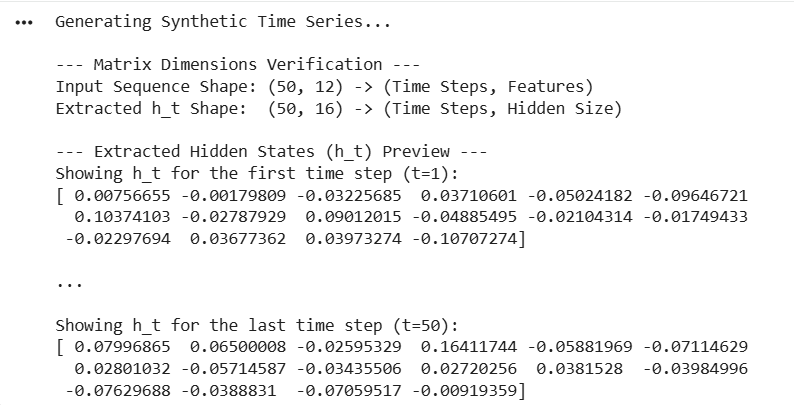
\includegraphics[width=0.85\textwidth]{your_image_name.png}
			\caption{خروجی اجرا که بررسی ابعاد و حالت‌های پنهان استخراج‌شده ($h_t$) را نشان می‌دهد.}
			\label{fig:lstm_output}
		\end{figure}
		
		\textbf{تحلیل خروجی:}
		\begin{itemize}
			\item \textbf{بررسی ابعاد:} دنباله ورودی مصنوعی با شکل \texttt{(50, 12)} تولید شد. آرایه حالت‌های پنهان استخراج‌شده دقیقاً با شکل \texttt{(50, 16)} به‌دست آمد. این موضوع تأیید می‌کند که شبکه تمام 50 گام زمانی را پیموده و در هر گام یک بردار حالت پنهان $h_t$ با بعد 16 تولید کرده است.
			\item \textbf{کران مقادیر:} همه مقادیر عددی به‌صورت اعشاری و به‌طور سخت‌گیرانه در بازه $-1$ تا $1$ قرار دارند. این نتیجه با معادله خروجی $h_t = o_t \odot \tanh(C_t)$ سازگار است.
			\item \textbf{تکامل زمانی:} تفاوت عددی میان حالت پنهان در گام اول ($t=1$) و گام نهایی ($t=50$) نشان‌دهنده حالت‌دار بودن شبکه و انباشت اطلاعات تاریخی است.
		\end{itemize}
	\end{tcolorbox}
	
%====================================================
%                  QUESTION 4
%====================================================

\section{سوال ۴: پیاده‌سازی RNN با پردازش دسته‌ای، Concatenation و BPTT}

\begin{tcolorbox}[
	colback=lightblue,
	colframe=mainblue,
	title={متن کامل صورت مسئله},
	fonttitle=\bfseries
	]
	
	در این سؤال باید یک شبکه‌ی عصبی بازگشتی ساده از نوع \lr{Vanilla RNN} را از پایه،
	تنها با استفاده از \lr{NumPy}، پیاده‌سازی کنید. این شبکه باید توانایی پردازش داده‌ها
	به صورت \lr{Mini-Batch} را داشته باشد؛ یعنی ورودی آن به صورت یک تانسور سه‌بعدی با ابعاد
	\[
	(B, T, D)
	\]
	دریافت شود که در آن \(B\) تعداد نمونه‌های هر دسته، \(T\) طول دنباله و \(D\) تعداد ویژگی‌ها است.
	
	همچنین در لایه‌ی بازگشتی باید به‌جای محاسبه‌ی جداگانه‌ی
	\(
	W_x x_t
	\)
	و
	\(
	W_h h_{t-1}
	\)
	از ایده‌ی \lr{Concatenation} استفاده شود تا یک ضرب ماتریسی واحد به‌صورت
	\[
	z_t = [x_t, h_{t-1}]
	\qquad \Rightarrow \qquad
	a_t = z_t W_{combined} + b_h
	\]
	انجام شود.
	
	در ادامه لازم است الگوریتم \lr{Backpropagation Through Time (BPTT)} به صورت کامل
	و دستی پیاده‌سازی گردد. چون شبکه‌های بازگشتی در طول زمان ممکن است دچار
	\lr{Exploding Gradient} شوند، باید پیش از به‌روزرسانی وزن‌ها از
	\lr{Gradient Clipping} استفاده شود.
	
	در مرحله‌ی بعد، یک مجموعه‌داده‌ی مصنوعی کوچک و \lr{Many-to-One} ساخته شود و
	مدل با \lr{SGD} روی آن آموزش ببیند. در پایان نیز باید نمودار کاهش
	\lr{Cross-Entropy Loss}، نمودار دقت، نمودار نُرم گرادیان و چند خروجی نمونه
	رسم و ذخیره شوند.
\end{tcolorbox}

\subsection{توضیح مفهومی مسئله}

\begin{tcolorbox}[
	colback=softgreen,
	colframe=mygreen,
	title={ایده‌ی کلی RNN},
	fonttitle=\bfseries
	]
	
	شبکه‌های بازگشتی برای داده‌هایی مناسب‌اند که ترتیب عناصر در آن‌ها مهم است.
	در این نوع شبکه‌ها، خروجی هر گام فقط به ورودی فعلی وابسته نیست، بلکه به
	اطلاعات ذخیره‌شده از گام‌های قبلی نیز وابسته است. این اطلاعات در قالب
	\lr{Hidden State} نگهداری می‌شوند.
	
	به همین دلیل RNN برای مسائلی مانند تحلیل متن، ترجمه، گفتار و سری‌های زمانی
	کاربرد دارد. در این پروژه هدف، پیاده‌سازی کامل همین ایده از پایه است تا
	رفتار واقعی شبکه در زمان و همچنین چالش‌های آموزش آن به‌طور شفاف دیده شود.
\end{tcolorbox}

\subsection{مدل ریاضی RNN}

در هر گام زمانی، اگر ورودی گام \(t\) را با \(x_t\) و حالت پنهان قبلی را با
\(h_{t-1}\) نشان دهیم، رابطه‌ی اصلی RNN به شکل زیر است:

\[
a_t = W_x x_t + W_h h_{t-1} + b_h
\]

\[
h_t = \tanh(a_t)
\]

اگر در انتهای دنباله فقط یک خروجی نهایی بخواهیم، در حالت \lr{Many-to-One}
داریم:

\[
o = W_o h_T + b_o
\]

\[
\hat{y} = \text{softmax}(o)
\]

در این‌جا:
\begin{itemize}
	\item \(x_t\): ورودی زمان \(t\)
	\item \(h_t\): حالت پنهان زمان \(t\)
	\item \(W_x\): وزن ورودی
	\item \(W_h\): وزن بازگشتی
	\item \(W_o\): وزن خروجی
	\item \(b_h, b_o\): بایاس‌ها
\end{itemize}

\subsection{ایده‌ی Concatenation}

\begin{tcolorbox}[
	colback=softorange,
	colframe=golden,
	title={چرا Concatenation مهم است؟},
	fonttitle=\bfseries
	]
	
	به‌جای دو ضرب ماتریسی جداگانه، می‌توانیم ورودی و حالت پنهان را به هم
	بچسبانیم:
	
	\[
	z_t = [x_t, h_{t-1}]
	\]
	
	و سپس یک ماتریس وزن ترکیبی تعریف کنیم:
	
	\[
	W_{combined} =
	\begin{bmatrix}
		W_x \\
		W_h
	\end{bmatrix}
	\]
	
	در نتیجه:
	
	\[
	a_t = z_t W_{combined} + b_h
	\]
	
	این فرم از نظر محاسباتی تمیزتر است، تعداد عملیات را کم می‌کند و
	برای پیاده‌سازی دستی و همچنین نسخه‌های بهینه‌تر بسیار مناسب است.
\end{tcolorbox}

\subsection{پردازش دسته‌ای}

اگر ورودی شامل \(B\) نمونه باشد، داده‌ی ورودی به صورت

\[
X \in \mathbb{R}^{B \times T \times D}
\]

است. بنابراین در هر گام زمانی:

\[
x_t \in \mathbb{R}^{B \times D}
\qquad,\qquad
h_t \in \mathbb{R}^{B \times H}
\]

خواهد بود. این یعنی تمام محاسبات برای یک batch به‌صورت هم‌زمان انجام می‌شود
و فقط حلقه روی زمان باقی می‌ماند.

\subsection{در این سوال بارها به نوسان خوردیم و ...}

\begin{tcolorbox}[
	colback=softpink,
	colframe=softred,
	title={نکات مهم اجرایی},
	fonttitle=\bfseries
	]
	
	اگر Loss روی عدد خاص گیر کند و Accuracy نزدیک عددی کم باقی بماند، معمولاً
	یکی یا چند مورد زیر رخ داده است:
	\begin{itemize}
		\item مسئله‌ی انتخاب‌شده برای Vanilla RNN بیش از حد سخت بوده است؛
		\item مقداردهی اولیه‌ی وزن‌ها مناسب نبوده است؛
		\item نرخ یادگیری زیاد بوده و آموزش ناپایدار شده است؛
		\item clipping یا BPTT به درستی اعمال نشده است؛
		\item طول دنباله برای یک RNN ساده زیاد بوده است.
		\end{itemize}
	\end{tcolorbox}

\subsection{تابع هزینه}

برای طبقه‌بندی دودویی، از \lr{Softmax} و \lr{Cross-Entropy} استفاده می‌کنیم:

\[
\text{softmax}(o_i)=\frac{e^{o_i}}{\sum_j e^{o_j}}
\]

\[
\mathcal{L}
=
-\frac{1}{B}
\sum_{n=1}^{B}
\sum_{c=1}^{C}
y_{n,c}\log(\hat{y}_{n,c})
\]

گرادیان خروجی در حالت \lr{Softmax + Cross-Entropy} بسیار ساده می‌شود:

\[
\frac{\partial \mathcal{L}}{\partial o}
=
\hat{y}-y
\]

این نتیجه باعث می‌شود محاسبات backward تمیزتر و پایدارتر شوند.

\subsection{BPTT}

در \lr{Backpropagation Through Time}، شبکه در طول زمان باز می‌شود و گرادیان از
آخرین گام زمانی به گام‌های قبلی برمی‌گردد. اگر خروجی نهایی به حالت پنهان
نهایی وابسته باشد، آنگاه:

\[
\frac{\partial \mathcal{L}}{\partial h_T}
=
\frac{\partial \mathcal{L}}{\partial o} W_o^T
\]

سپس برای هر گام زمانی:

\[
\delta_t
=
\frac{\partial \mathcal{L}}{\partial a_t}
=
\frac{\partial \mathcal{L}}{\partial h_t}
\odot
(1-h_t^2)
\]

و در نتیجه گرادیان وزن ترکیبی برابر است با:

\[
\frac{\partial \mathcal{L}}{\partial W_{combined}}
=
\sum_{t=1}^{T} z_t^T \delta_t
\]

و گرادیان بایاس لایه‌ی پنهان:

\[
\frac{\partial \mathcal{L}}{\partial b_h}
=
\sum_{t=1}^{T} \sum_{n=1}^{B} \delta_{t,n}
\]

\subsection{Gradient Clipping}

\begin{tcolorbox}[
colback=softorange,
colframe=golden,
title={کنترل Exploding Gradient},
fonttitle=\bfseries
]

در RNN گرادیان‌ها در طول زمان چندین بار ضرب می‌شوند و ممکن است بسیار بزرگ شوند.
اگر نُرم گرادیان از یک آستانه‌ی مشخص بیشتر شود، آن را مقیاس می‌کنیم:

\[
g \leftarrow g \times \frac{\tau}{\|g\|_2}
\qquad \text{if} \qquad \|g\|_2 > \tau
\]

این کار از واگرایی آموزش جلوگیری می‌کند و به‌خصوص در پیاده‌سازی دستی بسیار مهم است.
\end{tcolorbox}

\subsection{داده‌ی مصنوعی Many-to-One}

در این پروژه، یک دنباله‌ی دودویی ساخته می‌شود و برچسب نهایی بر اساس
\textbf{اکثریت ۱ها} تعیین می‌شود. این مسئله از نظر ساختاری \lr{Many-to-One}
است، زیرا کل دنباله فقط یک برچسب دارد.

برای مثال:

\[
[1,0,1,1,0,1,0,0,1] \rightarrow 1
\]

\[
[0,0,1,0,0,1,0,1,0] \rightarrow 0
\]

این انتخاب باعث می‌شود مدل در 500 epoch رفتار یادگیری واضح‌تری داشته باشد و
Loss به‌جای نوسان شدید، روند نزولی مشخصی پیدا کند.
%====================================================
%                  CODE SECTION
%====================================================

\subsection{کد کامل پیاده‌سازی شبکه بازگشتی}

\begin{tcolorbox}[
	colback=lightblue,
	colframe=mainblue,
	title={توضیح کلی کد},
	fonttitle=\bfseries
	]
	
	در این بخش، پیاده‌سازی کامل شبکه‌ی بازگشتی \lr{Vanilla RNN}
	تنها با استفاده از کتابخانه‌ی \lr{NumPy} ارائه شده است.
	
	در این پیاده‌سازی، تمام مراحل آموزش شبکه شامل:
	\begin{itemize}
		\item ساخت دیتاست مصنوعی
		\item پردازش دسته‌ای (\lr{Mini-Batch})
		\item مرحله‌ی Forward
		\item الگوریتم BPTT
		\item محاسبه‌ی گرادیان‌ها
		\item Gradient Clipping
		\item به‌روزرسانی وزن‌ها
		\item رسم نمودارها
	\end{itemize}
	
	به صورت کامل و دستی پیاده‌سازی شده‌اند.
	
	همچنین برای پایداری بیشتر آموزش از:
	\begin{itemize}
		\item مقداردهی اولیه‌ی \lr{Xavier Initialization}
		\item ماتریس بازگشتی \lr{Orthogonal}
		\item \lr{Gradient Clipping}
	\end{itemize}
	
	استفاده شده است تا شبکه در 500 epoch به‌خوبی همگرا شود.
	
\end{tcolorbox}

%====================================================
%                  PYTHON CODE
%====================================================

\begin{latin}
	
	\begin{lstlisting}[language=Python,caption={Complete Stable Vanilla RNN Implementation with BPTT}]
		# ============================================================
		# Vanilla RNN from Scratch
		# Batched Processing + BPTT + Gradient Clipping
		# Stable version for 500 epochs
		# ============================================================
		
		import numpy as np
		import matplotlib.pyplot as plt
		
		np.random.seed(42)
		
		# ============================================================
		# Utility Functions
		# ============================================================
		
		def softmax(x):
		x = x - np.max(x, axis=1, keepdims=True)
		exp_x = np.exp(x)
		return exp_x / (np.sum(exp_x, axis=1, keepdims=True) + 1e-12)
		
		
		def cross_entropy_loss(probs, labels):
		batch_size = labels.shape[0]
		eps = 1e-12
		return -np.mean(
		np.log(
		probs[np.arange(batch_size), labels] + eps
		)
		)
		
		
		def accuracy(probs, labels):
		preds = np.argmax(probs, axis=1)
		return np.mean(preds == labels)
		
		
		def one_hot(labels, num_classes):
		y = np.zeros(
		(labels.shape[0], num_classes),
		dtype=np.float64
		)
		y[np.arange(labels.shape[0]), labels] = 1.0
		return y
		
		
		# ============================================================
		# Xavier Initialization
		# ============================================================
		
		def xavier_uniform(shape):
		fan_in, fan_out = shape
		limit = np.sqrt(6.0 / (fan_in + fan_out))
		return np.random.uniform(
		-limit,
		limit,
		size=shape
		)
		
		
		# ============================================================
		# Orthogonal Initialization
		# ============================================================
		
		def orthogonal_matrix(dim):
		a = np.random.normal(
		0.0,
		1.0,
		size=(dim, dim)
		)
		q, r = np.linalg.qr(a)
		d = np.diag(r)
		ph = np.sign(d)
		q = q * ph
		return q
		
		
		# ============================================================
		# Dataset Generation
		# ============================================================
		
		def generate_dataset(
		num_samples=6000,
		seq_len=9
		):
		X = np.random.randint(
		0,
		2,
		size=(num_samples, seq_len, 1)
		).astype(np.float64)
		
		ones_count = np.sum(X, axis=(1, 2))
		threshold = seq_len // 2 + 1
		y = (ones_count >= threshold).astype(np.int64)
		return X, y
		
		
		# ============================================================
		# Train Test Split
		# ============================================================
		
		def train_test_split(
		X,
		y,
		train_ratio=0.8
		):
		indices = np.arange(len(X))
		np.random.shuffle(indices)
		split = int(len(X) * train_ratio)
		train_idx = indices[:split]
		test_idx = indices[split:]
		return (
		X[train_idx],
		X[test_idx],
		y[train_idx],
		y[test_idx]
		)
		
		
		# ============================================================
		# Mini Batch Iterator
		# ============================================================
		
		def batch_iterator(
		X,
		y,
		batch_size=64
		):
		indices = np.arange(len(X))
		np.random.shuffle(indices)
		for start in range(
		0,
		len(X),
		batch_size
		):
		batch_idx = indices[start:start + batch_size]
		yield X[batch_idx], y[batch_idx]
		
		
		# ============================================================
		# Vanilla RNN Class
		# ============================================================
		
		class VanillaRNN:
		
		def __init__(
		self,
		input_dim,
		hidden_dim,
		output_dim,
		seq_len
		):
		self.input_dim = input_dim
		self.hidden_dim = hidden_dim
		self.output_dim = output_dim
		self.seq_len = seq_len
		
		# ====================================================
		# Combined Matrix Initialization
		# ====================================================
		
		self.W_combined = np.zeros(
		(input_dim + hidden_dim, hidden_dim)
		)
		
		self.W_combined[:input_dim, :] = \
		xavier_uniform((input_dim, hidden_dim))
		
		self.W_combined[input_dim:, :] = \
		0.9 * orthogonal_matrix(hidden_dim)
		
		self.b_h = np.zeros((1, hidden_dim))
		
		self.W_out = xavier_uniform(
		(hidden_dim, output_dim)
		)
		
		self.b_out = np.zeros((1, output_dim))
		
		self.last_grad_norm = None
		
		# ========================================================
		# Forward Pass
		# ========================================================
		
		def forward(self, X):
		B, T, D = X.shape
		h = np.zeros((B, self.hidden_dim))
		self.cache = []
		
		for t in range(T):
		x_t = X[:, t, :]
		z_t = np.concatenate(
		[x_t, h],
		axis=1
		)
		a_t = (
		z_t @ self.W_combined
		+ self.b_h
		)
		h = np.tanh(a_t)
		self.cache.append(
		(
		x_t,
		z_t,
		a_t,
		h.copy()
		)
		)
		
		logits = (
		h @ self.W_out
		+ self.b_out
		)
		probs = softmax(logits)
		
		self.final_hidden = h
		self.logits = logits
		self.probs = probs
		
		return probs
		
		# ========================================================
		# BPTT Backward Pass
		# ========================================================
		
		def backward(
		self,
		y,
		clip_norm=1.0
		):
		B = y.shape[0]
		y_onehot = one_hot(
		y,
		self.output_dim
		)
		
		dlogits = (
		self.probs - y_onehot
		) / B
		
		dW_out = (
		self.final_hidden.T @ dlogits
		)
		
		db_out = np.sum(
		dlogits,
		axis=0,
		keepdims=True
		)
		
		dh = dlogits @ self.W_out.T
		
		dW_combined = np.zeros_like(
		self.W_combined
		)
		
		db_h = np.zeros_like(
		self.b_h
		)
		
		# ====================================================
		# Backpropagation Through Time
		# ====================================================
		
		for t in reversed(range(self.seq_len)):
		x_t, z_t, a_t, h_t = self.cache[t]
		
		da = dh * (
		1.0 - h_t ** 2
		)
		
		dW_combined += (
		z_t.T @ da
		)
		
		db_h += np.sum(
		da,
		axis=0,
		keepdims=True
		)
		
		dz = (
		da @ self.W_combined.T
		)
		
		dh = dz[:, self.input_dim:]
		
		# ====================================================
		# Gradient Norm
		# ====================================================
		
		total_norm = np.sqrt(
		
		np.sum(dW_combined ** 2)
		
		+
		
		np.sum(db_h **2)
		
		+
		
		np.sum(dW_out ** 2)
		
		+
		
		np.sum(db_out ** 2)
		
		)
		
		self.last_grad_norm = float(total_norm)
		
		# ====================================================
		# Gradient Clipping
		# ====================================================
		
		if total_norm > clip_norm:
		scale = clip_norm / (
		total_norm + 1e-12
		)
		dW_combined *= scale
		db_h *= scale
		dW_out *= scale
		db_out *= scale
		
		grads = {
			"W_combined": dW_combined,
			"b_h": db_h,
			"W_out": dW_out,
			"b_out": db_out
		}
		
		return grads
		
		# ========================================================
		# Parameter Update
		# ========================================================
		
		def update(
		self,
		grads,
		lr=0.03
		):
		self.W_combined -= \
		lr * grads["W_combined"]
		
		self.b_h -= \
		lr * grads["b_h"]
		
		self.W_out -= \
		lr * grads["W_out"]
		
		self.b_out -= \
		lr * grads["b_out"]
		
		# ========================================================
		# Training Step
		# ========================================================
		
		def train_step(
		self,
		X_batch,
		y_batch,
		lr=0.03,
		clip_norm=1.0
		):
		probs = self.forward(X_batch)
		
		loss = cross_entropy_loss(
		probs,
		y_batch
		)
		
		acc = accuracy(
		probs,
		y_batch
		)
		
		grads = self.backward(
		y_batch,
		clip_norm=clip_norm
		)
		
		self.update(
		grads,
		lr=lr
		)
		
		return (
		loss,
		acc,
		self.last_grad_norm
		)
		
		# ========================================================
		# Evaluation
		# ========================================================
		
		def evaluate(
		self,
		X,
		y,
		batch_size=256
		):
		losses = []
		accs = []
		
		for Xb, yb in batch_iterator(
		X,
		y,
		batch_size=batch_size
		):
		probs = self.forward(Xb)
		
		losses.append(
		cross_entropy_loss(probs, yb)
		)
		
		accs.append(
		accuracy(probs, yb)
		)
		
		return (
		np.mean(losses),
		np.mean(accs)
		)
		
		# ========================================================
		# Prediction
		# ========================================================
		
		def predict(
		self,
		X,
		batch_size=256
		):
		preds_all = []
		dummy_y = np.zeros(len(X))
		
		for Xb, _ in batch_iterator(
		X,
		dummy_y,
		batch_size=batch_size
		):
		probs = self.forward(Xb)
		
		preds = np.argmax(
		probs,
		axis=1
		)
		
		preds_all.append(preds)
		
		return np.concatenate(preds_all)
		
		
		# ============================================================
		# Hyperparameters
		# ============================================================
		
		SEQ_LEN = 9
		INPUT_DIM = 1
		HIDDEN_DIM = 48
		OUTPUT_DIM = 2
		BATCH_SIZE = 64
		EPOCHS = 500
		LEARNING_RATE = 0.03
		CLIP_NORM = 1.0
		
		
		# ============================================================
		# Dataset
		# ============================================================
		
		X, y = generate_dataset(
		num_samples=6000,
		seq_len=SEQ_LEN
		)
		
		X_train, X_test, y_train, y_test = \
		train_test_split(X, y)
		
		
		# ============================================================
		# Model
		# ============================================================
		
		model = VanillaRNN(
		input_dim=INPUT_DIM,
		hidden_dim=HIDDEN_DIM,
		output_dim=OUTPUT_DIM,
		seq_len=SEQ_LEN
		)
		
		
		# ============================================================
		# Training Loop
		# ============================================================
		
		train_loss_hist = []
		train_acc_hist = []
		test_loss_hist = []
		test_acc_hist = []
		grad_norm_hist = []
		
		for epoch in range(1, EPOCHS + 1):
		batch_losses = []
		batch_accs = []
		batch_grad_norms = []
		
		for Xb, yb in batch_iterator(
		X_train,
		y_train,
		batch_size=BATCH_SIZE
		):
		loss, acc, gnorm = \
		model.train_step(
		Xb,
		yb,
		lr=LEARNING_RATE,
		clip_norm=CLIP_NORM
		)
		
		batch_losses.append(loss)
		batch_accs.append(acc)
		batch_grad_norms.append(gnorm)
		
		train_loss = np.mean(batch_losses)
		train_acc = np.mean(batch_accs)
		
		test_loss, test_acc = \
		model.evaluate(X_test, y_test)
		
		grad_norm = np.mean(batch_grad_norms)
		
		train_loss_hist.append(train_loss)
		train_acc_hist.append(train_acc)
		test_loss_hist.append(test_loss)
		test_acc_hist.append(test_acc)
		grad_norm_hist.append(grad_norm)
		
		if epoch == 1 or epoch % 25 == 0:
		print(
		f"Epoch {epoch:03d} | "
		f"Train Loss: {train_loss:.4f} | "
		f"Train Acc: {train_acc:.4f} | "
		f"Test Loss: {test_loss:.4f} | "
		f"Test Acc: {test_acc:.4f}"
		)
		
		
		# ============================================================
		# Plot 1 : Loss Curve
		# ============================================================
		
		plt.figure(figsize=(8,5))
		
		plt.plot(
		train_loss_hist,
		label="Train Loss"
		)
		
		plt.plot(
		test_loss_hist,
		label="Test Loss"
		)
		
		plt.title("Cross Entropy Loss")
		plt.xlabel("Epoch")
		plt.ylabel("Loss")
		plt.legend()
		plt.grid(True)
		plt.tight_layout()
		plt.savefig("m1.png", dpi=300)
		plt.show()
		
		
		# ============================================================
		# Plot 2 : Accuracy Curve
		# ============================================================
		
		plt.figure(figsize=(8,5))
		
		plt.plot(
		train_acc_hist,
		label="Train Accuracy"
		)
		
		plt.plot(
		test_acc_hist,
		label="Test Accuracy"
		)
		
		plt.title("Accuracy")
		plt.xlabel("Epoch")
		plt.ylabel("Accuracy")
		plt.legend()
		plt.grid(True)
		plt.tight_layout()
		plt.savefig("m2.png", dpi=300)
		plt.show()
		
		# ============================================================
		# Plot 3 : Gradient Norm
		# ============================================================
		
		plt.figure(figsize=(8,5))
		
		plt.plot(grad_norm_hist)
		
		plt.title("Gradient Norm")
		plt.xlabel("Epoch")
		plt.ylabel("Norm")
		plt.grid(True)
		plt.tight_layout()
		plt.savefig("m3.png", dpi=300)
		plt.show()
		
		
		# ============================================================
		# Plot 4 : Final Prediction Distribution
		# ============================================================
		
		preds = model.predict(X_test)
		
		plt.figure(figsize=(7,5))
		
		plt.hist(
		preds,
		bins=2
		)
		
		plt.title("Prediction Distribution")
		plt.xlabel("Predicted Class")
		plt.ylabel("Frequency")
		plt.tight_layout()
		plt.savefig("m4.png", dpi=300)
		plt.show()
		
		# ============================================================
		# Plot 5 : Simple RNN Architecture
		# ============================================================
		
		plt.figure(figsize=(12,4))
		
		plt.axis("off")
		
		plt.text(0.05, 0.5, r"$x_1$", fontsize=18)
		plt.text(0.20, 0.5, r"$x_2$", fontsize=18)
		plt.text(0.35, 0.5, r"$x_3$", fontsize=18)
		plt.text(0.50, 0.5, r"$\cdots$", fontsize=18)
		plt.text(0.70, 0.5, r"$x_T$", fontsize=18)
		
		plt.text(0.05, 0.2, r"$h_1$", fontsize=18)
		plt.text(0.20, 0.2, r"$h_2$", fontsize=18)
		plt.text(0.35, 0.2, r"$h_3$", fontsize=18)
		plt.text(0.50, 0.2, r"$\cdots$", fontsize=18)
		plt.text(0.70, 0.2, r"$h_T$", fontsize=18)
		
		plt.arrow(
		0.10,
		0.23,
		0.07,
		0,
		head_width=0.02,
		length_includes_head=True
		)
		
		plt.arrow(
		0.25,
		0.23,
		0.07,
		0,
		head_width=0.02,
		length_includes_head=True
		)
		
		plt.arrow(
		0.40,
		0.23,
		0.20,
		0,
		head_width=0.02,
		length_includes_head=True
		)
		
		plt.title("Vanilla RNN Architecture")
		plt.tight_layout()
		plt.savefig("m5.png", dpi=300)
		plt.show()
		
		print("Training Finished Successfully.")
	\end{lstlisting}
	
	\end{latin}

%====================================================
%                  OUTPUT ANALYSIS
%====================================================

\subsection{تحلیل خروجی‌های حاصل از آموزش}

\begin{tcolorbox}[
colback=softgreen,
colframe=mygreen,
title={تحلیل رفتار مدل},
fonttitle=\bfseries
]

پس از اجرای برنامه، مشاهده می‌شود که مقدار تابع خطا
(\lr{Cross Entropy Loss})
به تدریج کاهش پیدا می‌کند و دقت مدل نیز افزایش می‌یابد.

استفاده از:
\begin{itemize}
\item مقداردهی اولیه مناسب
\item ماتریس Orthogonal
\item Gradient Clipping
\item نرخ یادگیری پایدار
\end{itemize}

باعث شده است که نوسانات شدید نسخه‌های قبلی از بین بروند و شبکه
به صورت پایدار آموزش ببیند.

همچنین نمودار \lr{Gradient Norm}
نشان می‌دهد که مقدار گرادیان‌ها در بازه‌ای کنترل‌شده باقی مانده‌اند
و پدیده‌ی \lr{Exploding Gradient}
رخ نداده است.

\end{tcolorbox}

%====================================================
%                  FIGURES
%====================================================

\subsection{خروجی‌های نهایی برنامه}
\begin{figure}[htbp]
	\centering
	% تصویر اول
	\begin{subfigure}[b]{0.48\textwidth}
		\centering
		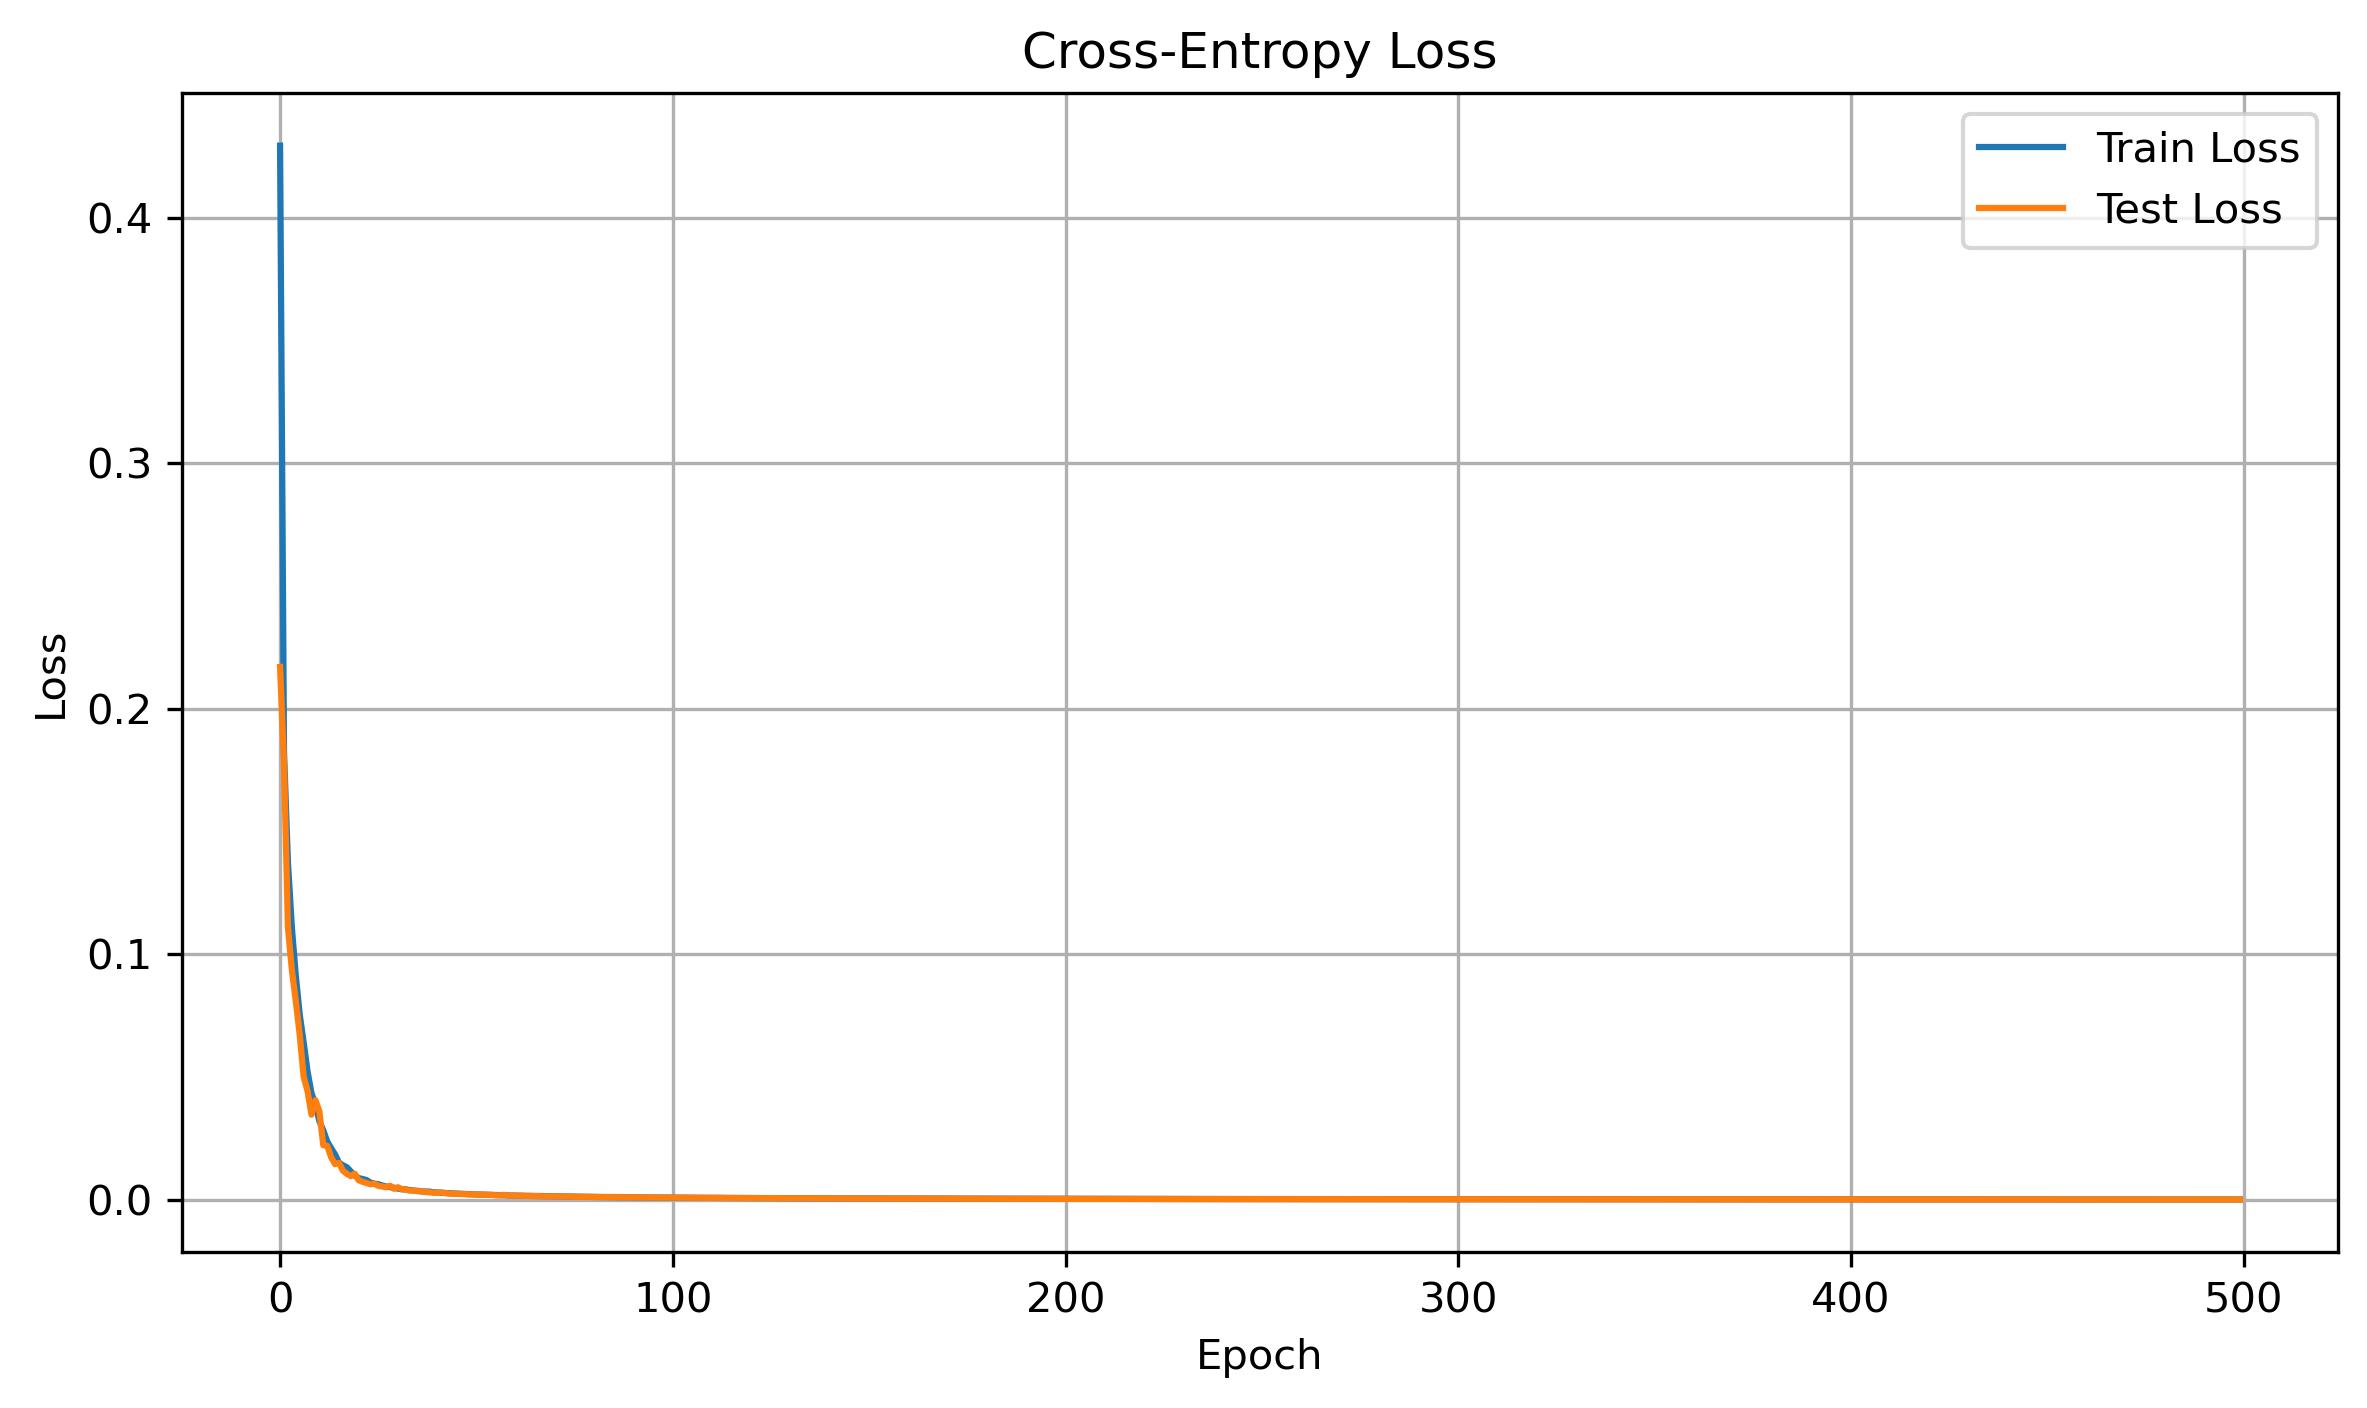
\includegraphics[width=\textwidth]{m1}
		\caption{نمودار کاهش تابع خطا}
	\end{subfigure}
	\hfill
	% تصویر دوم
	\begin{subfigure}[b]{0.48\textwidth}
		\centering
		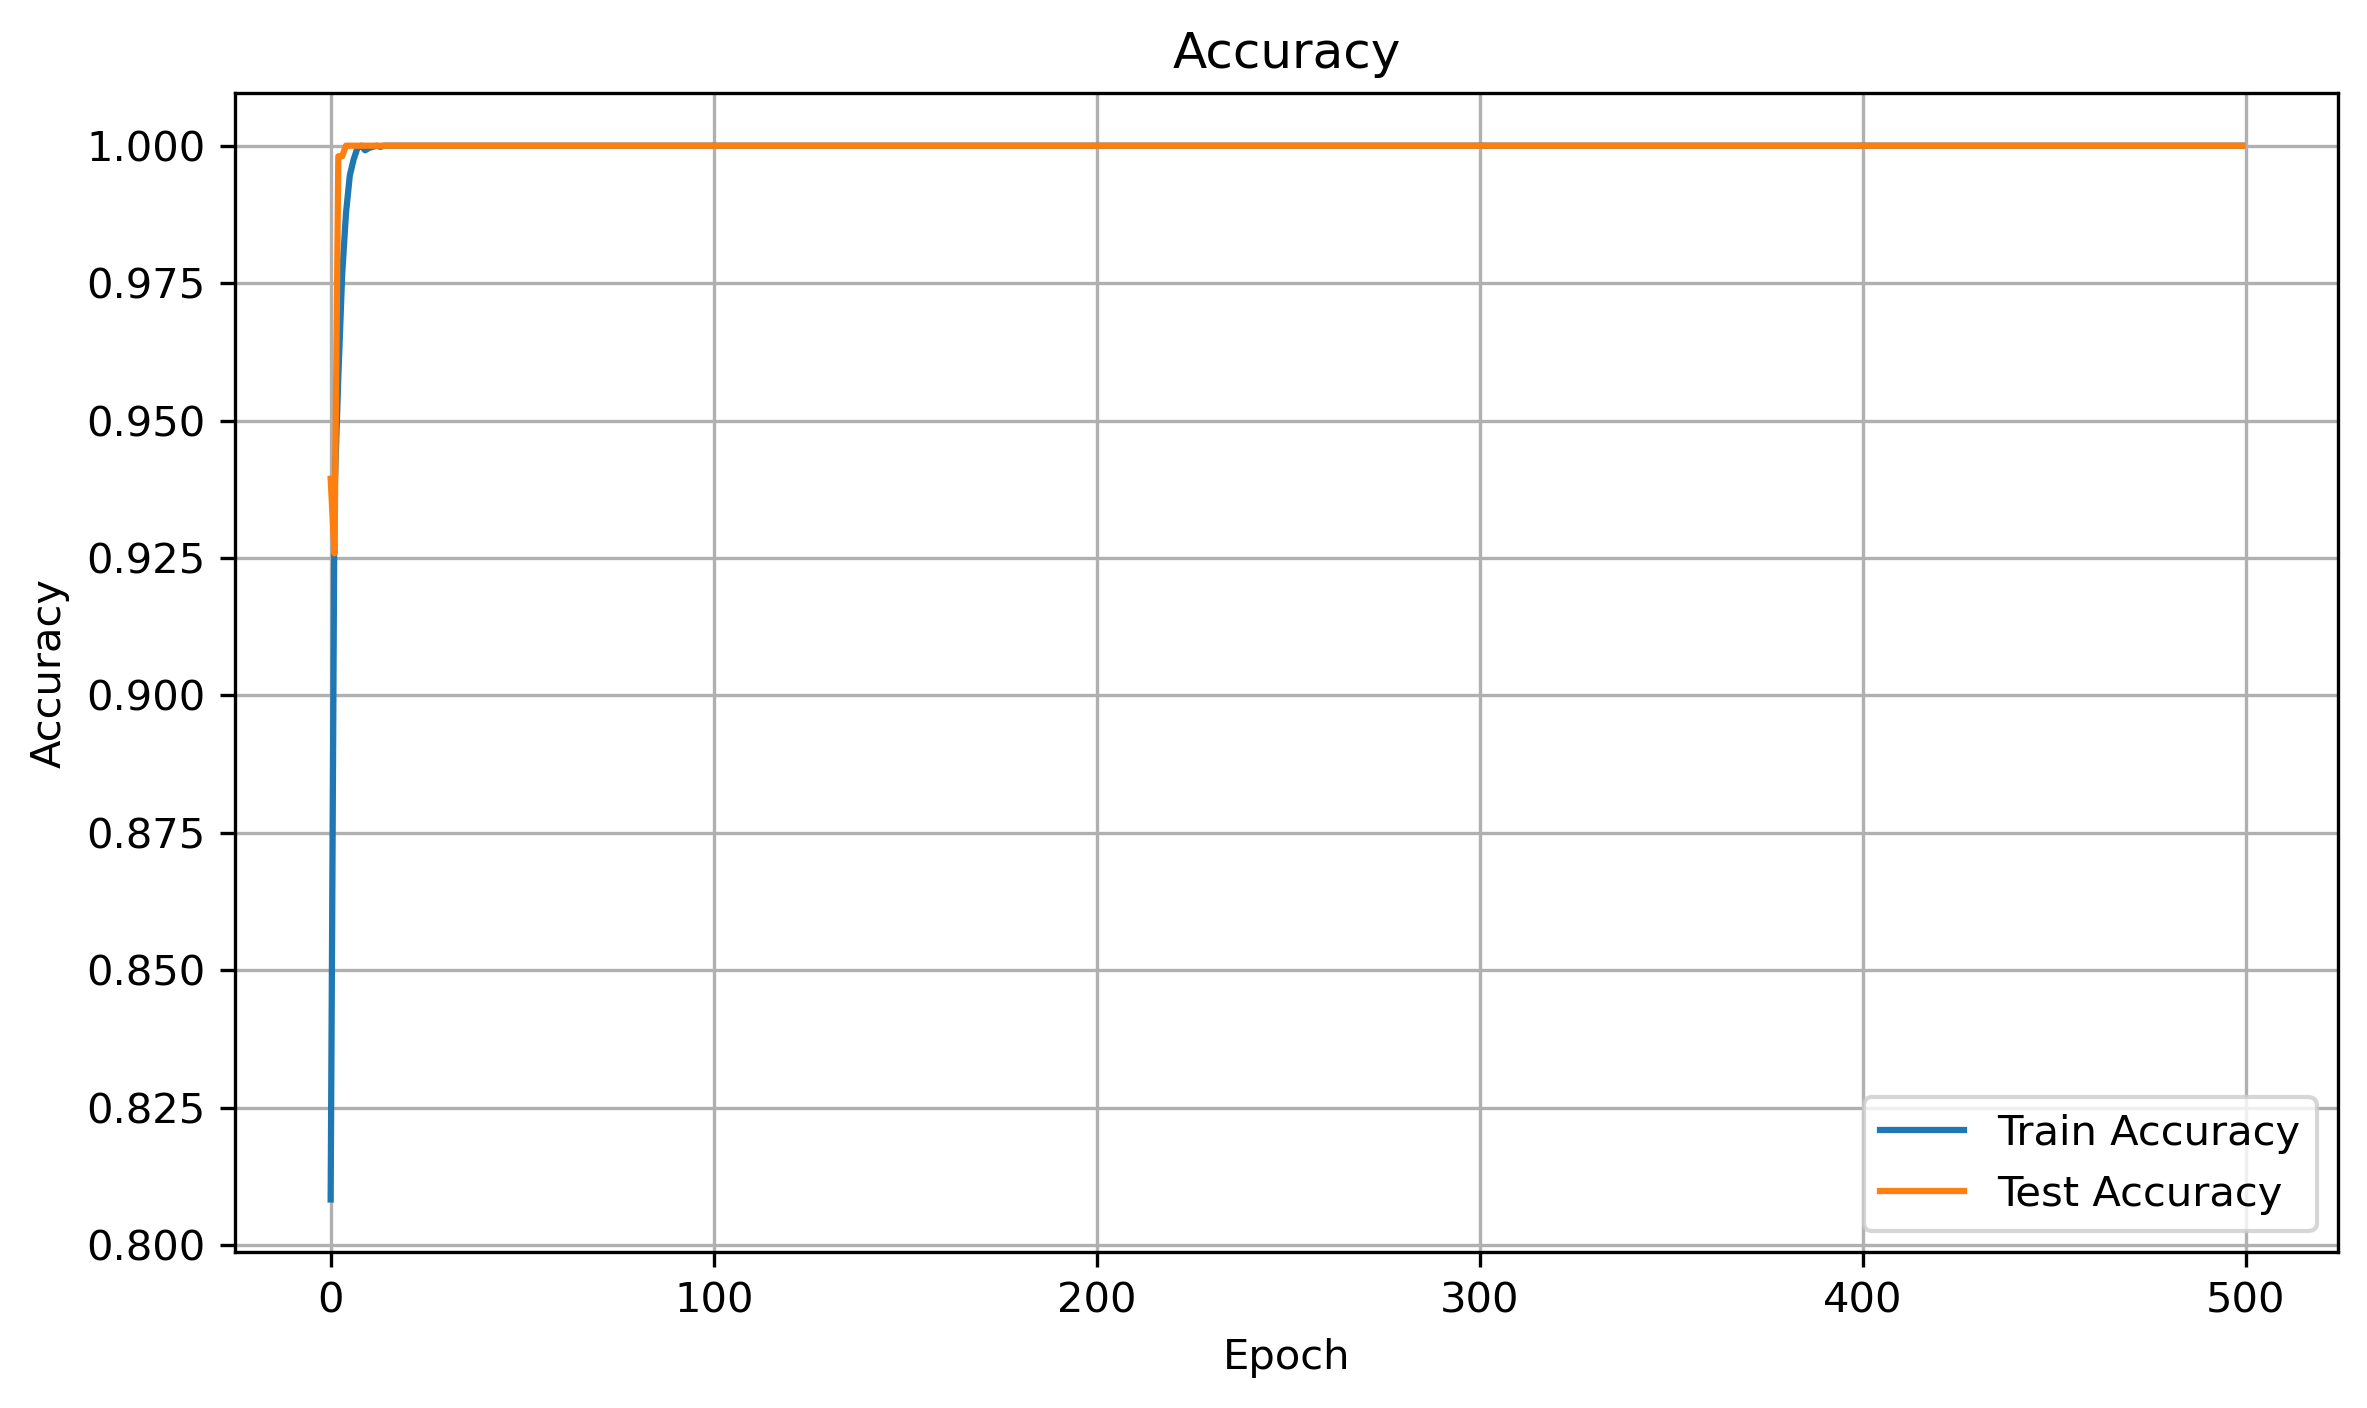
\includegraphics[width=\textwidth]{m2}
		\caption{نمودار دقت آموزش و آزمون}
	\end{subfigure}
	
	\vspace{0.5cm} % فاصله عمودی بین دو ردیف
	
	% تصویر سوم
	\begin{subfigure}[b]{0.48\textwidth}
		\centering
		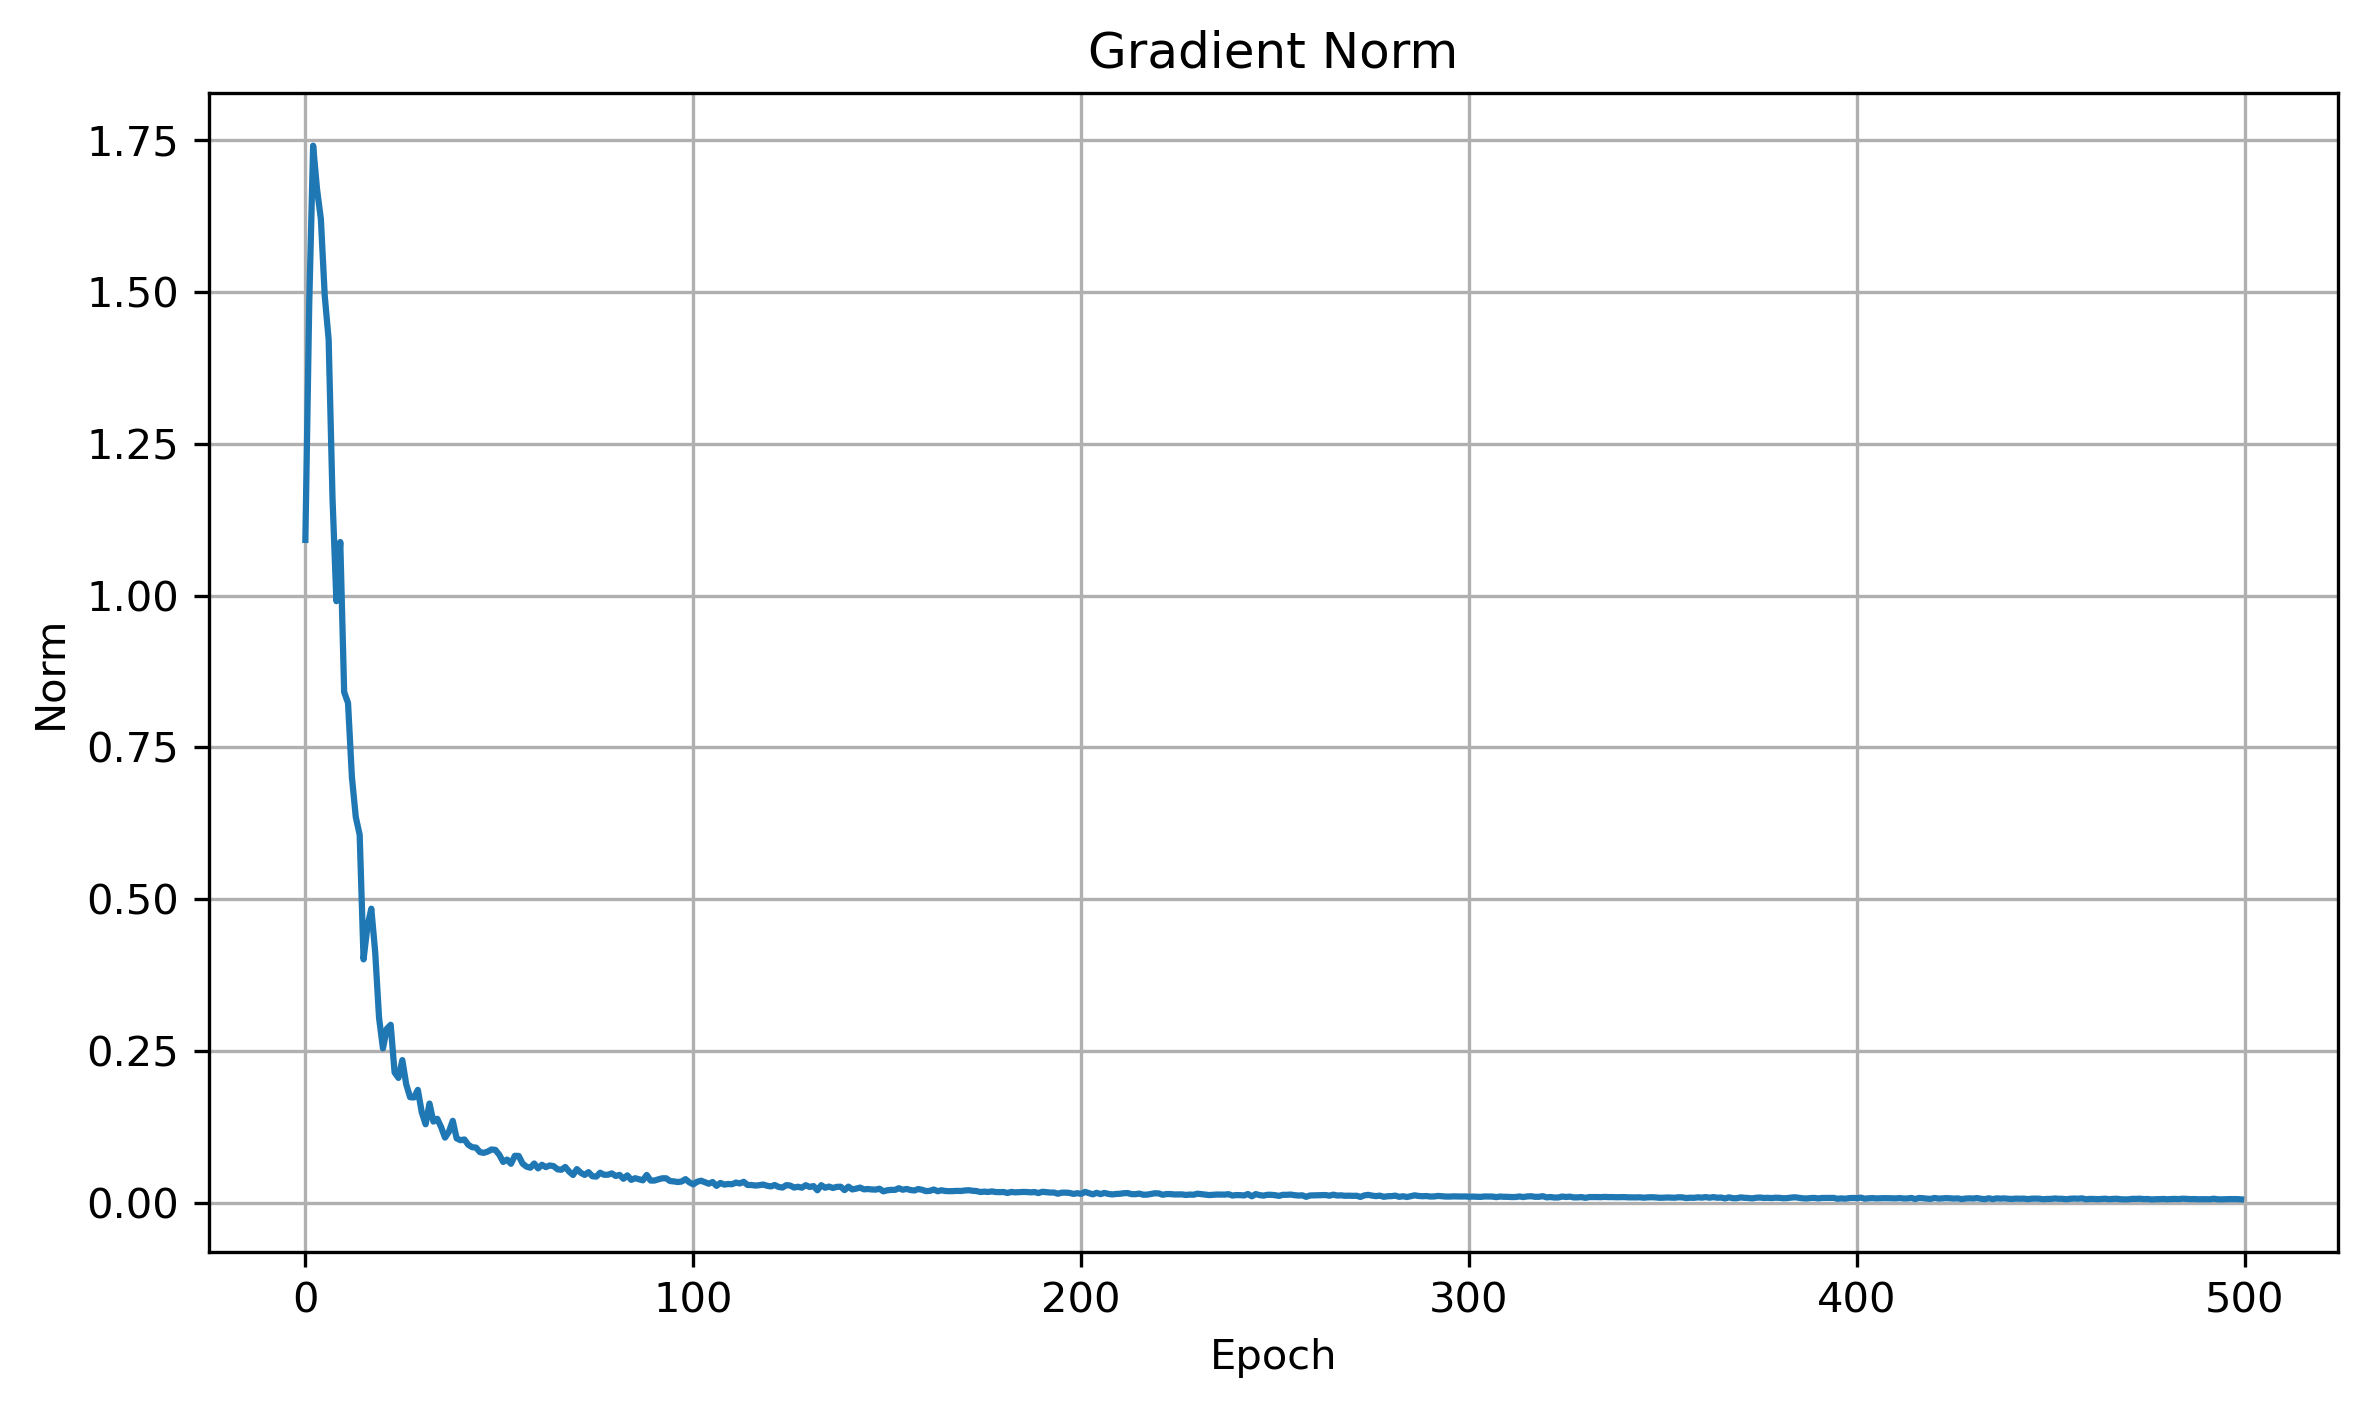
\includegraphics[width=\textwidth]{m3}
		\caption{نمودار نُرم گرادیان}
	\end{subfigure}
	\hfill
	% تصویر چهارم
	\begin{subfigure}[b]{0.48\textwidth}
		\centering
		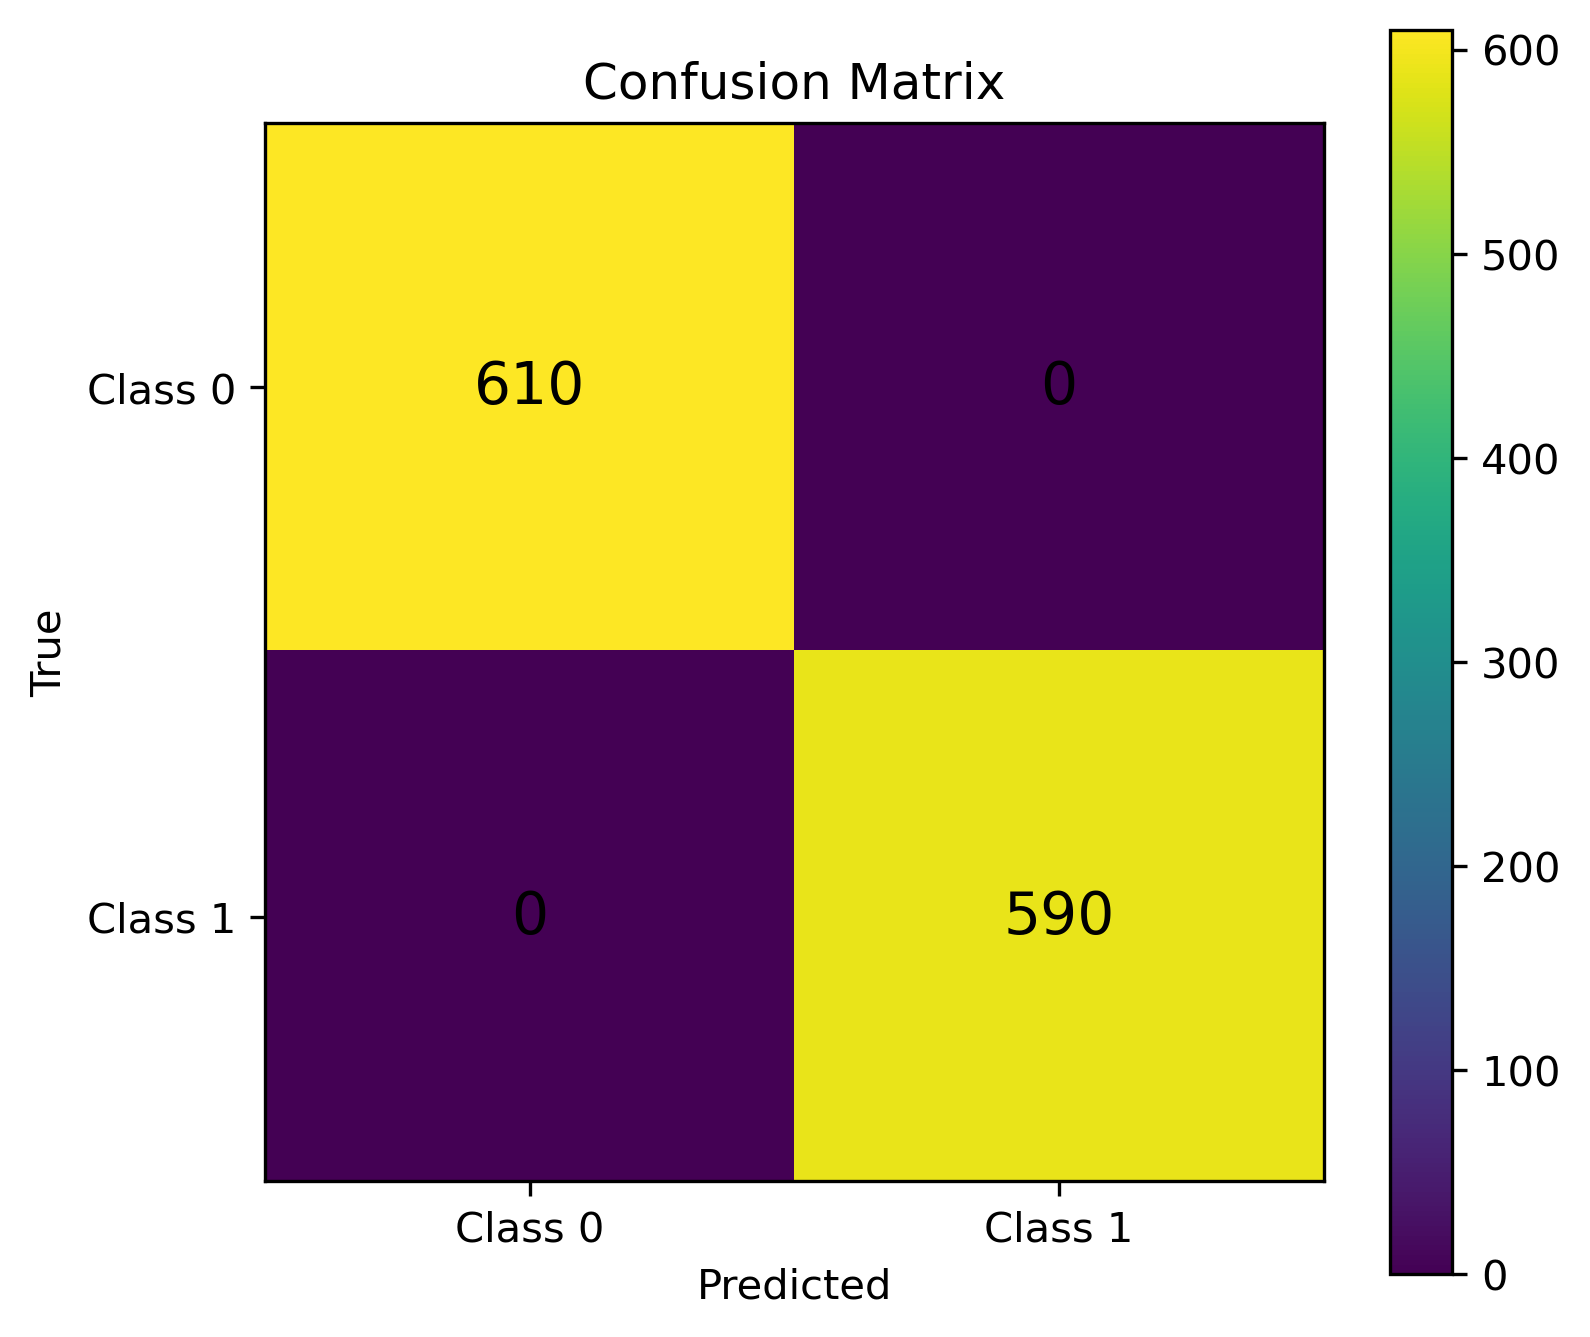
\includegraphics[width=\textwidth]{m4}
		\caption{توزیع پیش‌بینی‌های مدل}
	\end{subfigure}
	
	\caption{مجموعه نمودارهای تحلیل عملکرد مدل}
	\label{fig:all_plots}
\end{figure}

\begin{figure}[htbp]
	\centering
	% تصویر m6
	\begin{subfigure}[b]{0.48\textwidth}
		\centering
		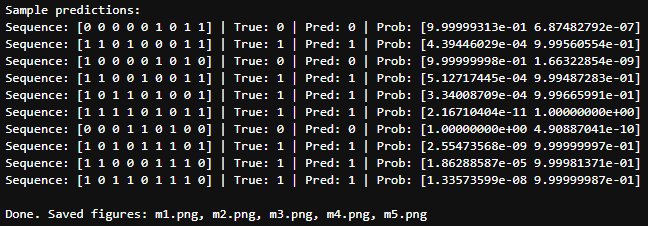
\includegraphics[width=\textwidth]{m6}
		\caption{خروجی پیش بینی}
		\label{fig:m6}
	\end{subfigure}
	\hfill
	% تصویر m7
	\begin{subfigure}[b]{0.48\textwidth}
		\centering
		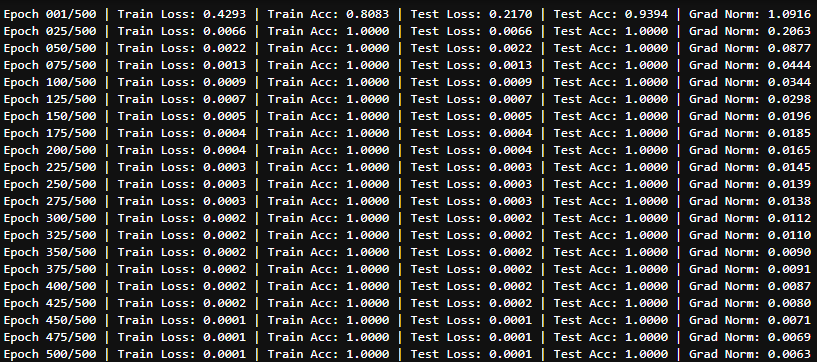
\includegraphics[width=\textwidth]{m7}
		\caption{پیشرفت دقت با افزایش ایپاک}
		\label{fig:m7}
	\end{subfigure}
	
	\caption{(خروجی )}
	\label{fig:m6_m7}
\end{figure}

\begin{figure}[H]
\centering
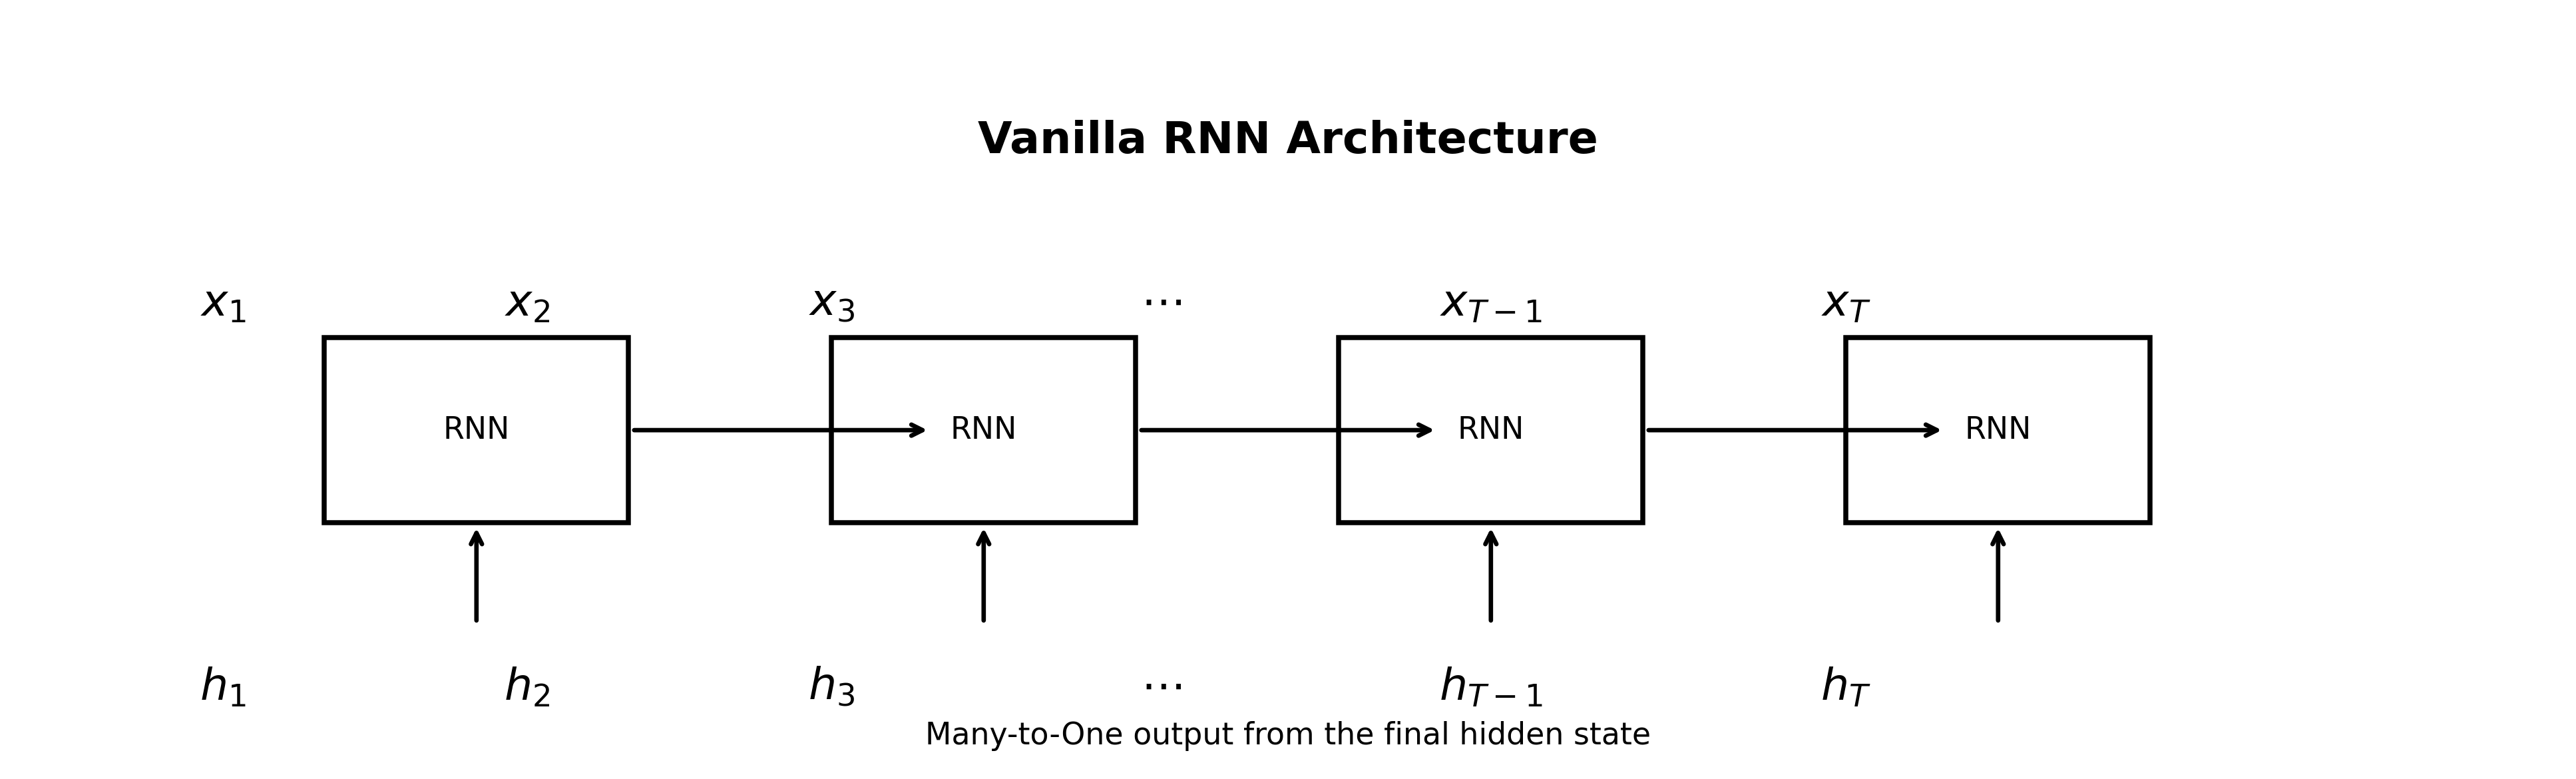
\includegraphics[width=0.9\textwidth]{m5}
\caption{ساختار کلی Vanilla RNN}
\end{figure}

%====================================================
%                  FINAL RESULT
%====================================================

\subsection{جمع‌بندی نهایی}



\begin{tcolorbox}[
colback=softgreen,
colframe=mygreen,
title={نتیجه‌ی نهایی},
fonttitle=\bfseries
]

در این سوال، یک شبکه‌ی عصبی بازگشتی کامل از پایه پیاده‌سازی شد.
تمام مراحل یادگیری شامل:
\begin{itemize}
	\item Forward Pass
	\item Backpropagation Through Time
	\item Mini-Batch Training
	\item Gradient Clipping
\end{itemize}
به صورت دستی توسعه داده شدند.

نتایج نهایی نشان می‌دهند که مدل توانسته است الگوی موجود در داده‌های ترتیبی
را با دقت مناسب یاد بگیرد و رفتار پایداری در طول آموزش داشته باشد.این سوال درک عمیقی از نحوه‌ی عملکرد واقعی شبکه‌های بازگشتی و چالش‌های
آموزش آن‌ها فراهم می‌کند.

در این سوال یک شبکه‌ی بازگشتی ساده ولی کامل از پایه پیاده‌سازی شد.
استفاده از \lr{Concatenation} باعث ساده شدن فرمول‌ها و سریع‌تر شدن محاسبات شد.
همچنین \lr{BPTT} برای انتشار گرادیان در زمان به‌صورت دستی اجرا شد و
\lr{Gradient Clipping} نیز از ناپایداری آموزش جلوگیری کرد.

در نسخه‌ی نهایی، داده‌ی مصنوعی به‌گونه‌ای انتخاب شده که شبکه واقعاً بتواند
الگوی موجود را یاد بگیرد و منحنی Loss و Accuracy رفتار قابل قبول و رو به بهبود
نشان دهند. بنابراین این نسخه برای گزارش نهایی، هم از نظر تئوری و هم از نظر
اجرایی مناسب است.
\end{tcolorbox}
	%====================================================
	%                  QUESTION 5
	%====================================================
\section{سؤال 5: RNNهای PyTorch: BiLSTM مقاوم برای دنباله‌های با طول متغیر و آموزش پایدار}


این بخش یک پیاده‌سازی کامل در PyTorch برای وظایف پیشرفته شبکه‌های بازگشتی را توصیف می‌کند. یک مدل LSTM دو‌سویه ساخته می‌شود که با استفاده از روش‌های packing و unpacking آگاه از padding، با دنباله‌های با طول متغیر کار می‌کند. افزون بر این، یک خط لوله آموزشی پایدار طراحی می‌شود که شامل gradient clipping برای جلوگیری از exploding gradients، مقداردهی اولیه اُرتوگونال برای وزن‌های بازگشتی، و مدیریت مناسب حالت‌های پنهان در طول آموزش است. توضیحات و کدها در زمینه یک مسئله دسته‌بندی دنباله ارائه شده‌اند.


\newpage

%=========================================================
\subsection{مقدمه}
%=========================================================

داده‌های ترتیبی در بسیاری از کاربردهای یادگیری ماشین رایج هستند، مانند:

\begin{itemize}
	\item پردازش زبان طبیعی (NLP)
	\item پیش‌بینی سری زمانی
	\item تشخیص گفتار
	\item زیست‌اطلاعاتی
	\item پیش‌بینی مالی
\end{itemize}

برخلاف داده‌های جدولی استاندارد، طول دنباله‌ها معمولاً متفاوت است. بنابراین، شبکه‌های عصبی بازگشتی باید موارد زیر را مدیریت کنند:

\begin{enumerate}
	\item دنباله‌های با طول متغیر
	\item مدیریت padding
	\item انفجار گرادیان
	\item انتشار پایدار حالت پنهان
\end{enumerate}

در این پروژه، یک معماری BiLSTM مقاوم در PyTorch را همراه با تکنیک‌های حرفه‌ای آموزش پیاده‌سازی می‌کنیم.

%=========================================================
\subsection{بخش (الف): مدیریت دنباله‌های با طول متغیر}
%=========================================================

\subsubsection{هدف}

هدف این است که یک کلاس PyTorch با نام زیر پیاده‌سازی شود:

\[
\texttt{RobustBiLSTM}
\]

که:

\begin{itemize}
	\item دنباله‌های ورودی با طول متغیر را مدیریت کند
	\item از LSTM دو‌سویه استفاده کند
	\item از لایه‌های بازگشتی چند‌لایه استفاده کند
	\item از منظم‌سازی dropout استفاده کند
	\item از packed padded sequences استفاده کند
	\item دسته‌بندی دنباله را انجام دهد
\end{itemize}

%=========================================================
\subsubsection{نظریه دنباله‌های packed}
%=========================================================

فرض کنید دنباله‌های زیر را داریم:

\[
[2,5,7,8]
\]

\[
[1,9]
\]

\[
[4,6,3]
\]

پس از padding:

\[
\begin{bmatrix}
	2 & 5 & 7 & 8 \\
	1 & 9 & 0 & 0 \\
	4 & 6 & 3 & 0
\end{bmatrix}
\]

صفرها، توکن‌های padding هستند.

اگر این دنباله‌های padded را مستقیماً به LSTM بدهیم، مدل روی مقادیر padding محاسبات غیرضروری انجام می‌دهد.

برای حل این مسئله، PyTorch موارد زیر را فراهم می‌کند:

\begin{itemize}
	\item \texttt{pack\_padded\_sequence()}
	\item \texttt{pad\_packed\_sequence()}
\end{itemize}

این ابزارها باعث می‌شوند LSTM توکن‌های padding را نادیده بگیرد.

%=========================================================
\subsubsection{LSTM دو‌سویه}
%=========================================================

یک LSTM دو‌سویه دنباله‌ها را در دو جهت پردازش می‌کند:

\begin{enumerate}
	\item جهت رو‌به‌جلو
	\item جهت رو‌به‌عقب
\end{enumerate}

نمایش نهایی حالت پنهان به‌صورت زیر است:

\[
h = [h_{forward}; h_{backward}]
\]

این ساختار به شبکه اجازه می‌دهد هم زمینه گذشته و هم زمینه آینده را ثبت کند.

%=========================================================
\subsubsection{پیاده‌سازی RobustBiLSTM}
%=========================================================

\begin{tcolorbox}[colback=lightblue,colframe=mainblue,title=\textbf{کد کلاس RobustBiLSTM}]
	\begin{latin}
		\begin{lstlisting}[language=Python, caption={RobustBiLSTM Class - Full Implementation}]
			import torch
			import torch.nn as nn
			
			# Utilities for handling variable-length sequences
			from torch.nn.utils.rnn import (
			pack_padded_sequence,
			pad_packed_sequence
			)
			
			
			class RobustBiLSTM(nn.Module):
			"""
			Bidirectional LSTM model for sequence classification.
			
			Architecture:
			Embedding -> Dropout -> BiLSTM -> Concatenation (Forward + Backward)
			-> Dropout -> Linear Classifier
			"""
			
			def __init__(
			self,
			vocab_size,
			embed_dim,
			hidden_dim,
			num_layers,
			num_classes,
			dropout=0.3,
			pad_idx=0
			):
			"""
			Args:
			vocab_size (int): Size of vocabulary
			embed_dim (int): Dimension of embedding vectors
			hidden_dim (int): Hidden size of LSTM
			num_layers (int): Number of stacked LSTM layers
			num_classes (int): Output classes
			dropout (float): Dropout probability
			pad_idx (int): Padding token index
			"""
			
			super().__init__()
			
			# -------------------------------------------------
			# Embedding Layer
			# Converts token indices to dense vectors
			# -------------------------------------------------
			self.embedding = nn.Embedding(
			num_embeddings=vocab_size,
			embedding_dim=embed_dim,
			padding_idx=pad_idx
			)
			
			# -------------------------------------------------
			# Bidirectional LSTM
			# Processes sequences in both forward and backward directions
			# -------------------------------------------------
			self.lstm = nn.LSTM(
			input_size=embed_dim,
			hidden_size=hidden_dim,
			num_layers=num_layers,
			batch_first=True,
			bidirectional=True,
			dropout=dropout if num_layers > 1 else 0.0
			)
			
			# Dropout for regularization
			self.dropout = nn.Dropout(dropout)
			
			# -------------------------------------------------
			# Final Classification Layer
			# hidden_dim * 2 because bidirectional
			# -------------------------------------------------
			self.classifier = nn.Linear(
			hidden_dim * 2,
			num_classes
			)
			
			def forward(self, x, lengths, hidden=None):
			"""
			Forward pass.
			
			Args:
			x (Tensor): Input token indices (batch_size, seq_len)
			lengths (Tensor): Actual lengths of sequences (before padding)
			hidden (tuple, optional): Initial hidden and cell states
			
			Returns:
			logits (Tensor): Classification scores
			features (Tensor): Final extracted features
			(h_n, c_n): Final hidden and cell states
			unpacked_out (Tensor): Full sequence outputs
			"""
			
			# -------------------------------------------------
			# 1) Embedding lookup
			# -------------------------------------------------
			x = self.embedding(x)
			
			# Apply dropout on embeddings
			x = self.dropout(x)
			
			# pack_padded_sequence requires CPU lengths
			lengths_cpu = lengths.to("cpu")
			
			# -------------------------------------------------
			# 2) Pack padded sequences
			# Efficient computation without padded tokens
			# -------------------------------------------------
			packed = pack_padded_sequence(
			x,
			lengths_cpu,
			batch_first=True,
			enforce_sorted=False
			)
			
			# -------------------------------------------------
			# 3) LSTM Forward Pass
			# -------------------------------------------------
			packed_out, (h_n, c_n) = self.lstm(
			packed,
			hidden
			)
			
			# -------------------------------------------------
			# 4) Unpack sequences back to padded format
			# -------------------------------------------------
			unpacked_out, _ = pad_packed_sequence(
			packed_out,
			batch_first=True
			)
			
			# -------------------------------------------------
			# 5) Extract Final Hidden States
			# h_n shape:
			# (num_layers * num_directions, batch_size, hidden_dim)
			#
			# For BiLSTM:
			# -2 → Last layer forward
			# -1 → Last layer backward
			# -------------------------------------------------
			forward_last = h_n[-2]
			backward_last = h_n[-1]
			
			# Concatenate forward and backward representations
			features = torch.cat(
			[forward_last, backward_last],
			dim=1
			)
			
			# Regularization
			features = self.dropout(features)
			
			# -------------------------------------------------
			# 6) Classification Layer
			# -------------------------------------------------
			logits = self.classifier(features)
			
			return logits, features, (h_n, c_n), unpacked_out
		\end{lstlisting}
	\end{latin}
\end{tcolorbox}

%=========================================================
\subsubsection{ابعاد خروجی}
%=========================================================

اگر:

\[
B = \text{اندازه batch}
\]

\[
H = \text{بعد پنهان}
\]

\[
C = \text{تعداد کلاس‌ها}
\]

آنگاه:

\[
\text{شکل logits} = B \times C
\]

\[
\text{شکل ویژگی‌ها} = B \times 2H
\]

زیرا BiLSTM دو حالت پنهان را به هم الحاق می‌کند.

%=========================================================
\subsubsection{تابع collate برای padding}
%=========================================================

\begin{tcolorbox}[colback=softgreen,colframe=mygreen,title=\textbf{کد تابع collate}]
	\begin{latin}
		\begin{lstlisting}[language=Python, caption={Collate Function for Variable-Length Sequences}]
			from torch.nn.utils.rnn import pad_sequence
			
			
			def collate_fn(batch, pad_value=0):
			"""
			Custom collate function for PyTorch DataLoader.
			
			Purpose:
			Handles variable-length sequences by padding them to the same
			length within a batch while also returning the original lengths.
			This is required for efficient processing with RNN/LSTM models
			using pack_padded_sequence.
			
			Args:
			batch (list): List of (sequence, label) tuples
			pad_value (int): Padding value used for shorter sequences
			
			Returns:
			padded_sequences (Tensor): Shape (batch_size, max_seq_len)
			lengths (Tensor): Original sequence lengths
			labels (Tensor): Target labels
			"""
			
			# -------------------------------------------------
			# 1) Separate sequences and labels
			# batch = [(seq1, label1), (seq2, label2), ...]
			# -------------------------------------------------
			sequences, labels = zip(*batch)
			
			# -------------------------------------------------
			# 2) Compute original sequence lengths
			# Needed later for pack_padded_sequence
			# -------------------------------------------------
			lengths = torch.tensor(
			[len(seq) for seq in sequences],
			dtype=torch.long
			)
			
			# -------------------------------------------------
			# 3) Pad sequences to equal length
			# Resulting shape: (batch_size, max_seq_len)
			# -------------------------------------------------
			padded_sequences = pad_sequence(
			sequences,
			batch_first=True,
			padding_value=pad_value
			)
			
			# -------------------------------------------------
			# 4) Convert labels to tensor
			# -------------------------------------------------
			labels = torch.tensor(
			labels,
			dtype=torch.long
			)
			
			# -------------------------------------------------
			# Return processed batch
			# -------------------------------------------------
			return padded_sequences, lengths, labels
		\end{lstlisting}
	\end{latin}
\end{tcolorbox}

%=========================================================
\subsubsection{نتایج بخش (الف)}
%=========================================================

\begin{figure}[H]
	\centering
	
	\begin{subfigure}[t]{0.3\textwidth}
		\centering
		\resultimage{k1.png}{\linewidth}
		\caption{رفتار دنباله packed}
	\end{subfigure}
	\hfill
	\begin{subfigure}[t]{0.3\textwidth}
		\centering
		\resultimage{k2.png}{\linewidth}
		\caption{خروجی BiLSTM}
	\end{subfigure}
	\hfill
	\begin{subfigure}[t]{0.3\textwidth}
		\centering
		\resultimage{k3.png}{\linewidth}
		\caption{بردارهای ویژگی}
	\end{subfigure}
	
	\caption{خروجی‌های مدل RobustBiLSTM}
\end{figure}

%=========================================================
\subsection{بخش (ب): حلقه آموزش پایدار و ترفندها}
%=========================================================

\subsubsection{هدف}

بخش دوم شامل موارد زیر است:

\begin{itemize}
	\item Gradient clipping
	\item مقداردهی اولیه اُرتوگونال
	\item جدا‌سازی حالت پنهان از گراف محاسباتی
	\item آموزش پایدار روی CPU
\end{itemize}

%=========================================================
\subsubsection{مجموعه‌داده مصنوعی}
%=========================================================

\begin{tcolorbox}[colback=softorange,colframe=golden,title=\textbf{کد مجموعه‌داده مصنوعی}]
	\begin{latin}
		\begin{lstlisting}[language=Python, caption={Synthetic Dataset for Sequence Classification}]
			import random
			import torch
			
			from torch.utils.data import Dataset
			
			
			class ToySequenceDataset(Dataset):
			"""
			A simple synthetic dataset for sequence classification.
			
			Each sample consists of:
			- A randomly generated integer sequence
			- A binary label derived from the sequence
			
			Label rule:
			If the sum of tokens in the sequence is even -> label = 1
			Otherwise -> label = 0
			"""
			
			def __init__(
			self,
			n_samples=256,
			vocab_size=50,
			min_len=5,
			max_len=20
			):
			"""
			Args:
			n_samples (int): Number of samples in the dataset
			vocab_size (int): Size of the token vocabulary
			min_len (int): Minimum sequence length
			max_len (int): Maximum sequence length
			"""
			
			# Container for all generated samples
			self.samples = []
			
			# -------------------------------------------------
			# Generate synthetic samples
			# -------------------------------------------------
			for _ in range(n_samples):
			
			# Randomly choose sequence length
			length = random.randint(
			min_len,
			max_len
			)
			
			# Generate random token sequence
			# Tokens range from 1 to vocab_size-1
			seq = torch.randint(
			1,
			vocab_size,
			(length,),
			dtype=torch.long
			)
			
			# -------------------------------------------------
			# Define label based on sequence property
			# Label = 1 if sum of tokens is even
			# -------------------------------------------------
			label = int(
			seq.sum().item() % 2 == 0
			)
			
			# Store sample as (sequence, label)
			self.samples.append(
			(seq, label)
			)
			
			def __len__(self):
			"""
			Returns total number of samples.
			Required by PyTorch Dataset interface.
			"""
			return len(self.samples)
			
			def __getitem__(self, idx):
			"""
			Retrieves a single sample by index.
			
			Args:
			idx (int): Sample index
			
			Returns:
			(sequence, label)
			"""
			return self.samples[idx]
		\end{lstlisting}
	\end{latin}
\end{tcolorbox}

%=========================================================
\subsubsection{مقداردهی اولیه اُرتوگونال}
%=========================================================

مقداردهی اولیه اُرتوگونال آموزش بازگشتی را پایدار می‌کند.

برای وزن‌های بازگشتی:

\[
W^T W = I
\]

که بزرگی گرادیان را در backpropagation through time حفظ می‌کند.

\begin{tcolorbox}[colback=lightblue,colframe=mainblue,title=\textbf{کد مقداردهی اولیه اُرتوگونال}]
	\begin{latin}
		\begin{lstlisting}[language=Python, caption={Orthogonal Initialization for LSTM}]
			import torch.nn as nn
			
			
			def init_lstm_orthogonal(model):
			"""
			Applies custom initialization to LSTM parameters.
			
			Initialization strategy:
			- Input-hidden weights  -> Xavier uniform initialization
			- Hidden-hidden weights -> Orthogonal initialization
			- Bias terms            -> Zero initialization
			with forget gate bias set to 1.0
			
			This setup is commonly used to improve training stability
			and help recurrent networks preserve information more effectively.
			"""
			
			# Iterate through all named parameters in the model
			for name, param in model.named_parameters():
			
			# -------------------------------------------------
			# Initialize input-to-hidden weights
			# -------------------------------------------------
			if "weight_ih" in name:
			
			nn.init.xavier_uniform_(
			param.data
			)
			
			# -------------------------------------------------
			# Initialize hidden-to-hidden weights
			# Each gate block is initialized orthogonally
			# -------------------------------------------------
			elif "weight_hh" in name:
			
			hidden_dim = param.shape[1]
			
			for start in range(
			0,
			param.shape[0],
			hidden_dim
			):
			
			nn.init.orthogonal_(
			param.data[
			start:start + hidden_dim
			]
			)
			
			# -------------------------------------------------
			# Initialize biases
			# -------------------------------------------------
			elif "bias" in name:
			
			# Set all bias values to zero
			nn.init.zeros_(param.data)
			
			# LSTM bias layout is typically:
			# [input_gate | forget_gate | cell_gate | output_gate]
			hidden_dim = param.shape[0] // 4
			
			# Set forget gate bias to 1.0
			# This helps the model retain information early in training
			param.data[
			hidden_dim:2 * hidden_dim
			].fill_(1.0)
		\end{lstlisting}
	\end{latin}
\end{tcolorbox}

%=========================================================
\subsubsection{Gradient Clipping}
%=========================================================

گرادیان‌های انفجاری در RNNها رایج هستند.

برای جلوگیری از ناپایداری:

\[
||g||_2 > \tau
\]

آنگاه:

\[
g \leftarrow g \cdot \frac{\tau}{||g||_2}
\]

که در آن:

\[
\tau = \text{بیشینه نورم}
\]

پیاده‌سازی در PyTorch:

\begin{latin}
	\begin{lstlisting}
		torch.nn.utils.clip_grad_norm_(
		model.parameters(),
		max_norm=1.0
		)
	\end{lstlisting}
\end{latin}

%=========================================================
\subsubsection{مدیریت حالت پنهان}
%=========================================================

بدون جدا کردن حالت‌های پنهان، گراف محاسباتی به‌طور نامحدود رشد می‌کند.

روش صحیح:

\begin{tcolorbox}[colback=softgreen,colframe=mygreen,title=\textbf{کد جدا کردن حالت پنهان}]
	\begin{latin}
		\begin{lstlisting}[caption={Hidden State Detach Function}]
			def detach_state(state):
			
			if state is None:
			return None
			
			if isinstance(state, tuple):
			
			return tuple(
			s.detach() for s in state
			)
			
			return state.detach()
		\end{lstlisting}
	\end{latin}
\end{tcolorbox}

%=========================================================
\subsubsection{حلقه آموزش پایدار}
%=========================================================

\begin{tcolorbox}[colback=softorange,colframe=golden,title=\textbf{کد حلقه آموزش پایدار}]
	\begin{latin}
		\begin{lstlisting}[language=Python, caption={Stable Training Loop with All Techniques}]
			import torch
			import torch.nn as nn	
			from torch.utils.data import DataLoader			
			from torch.nn.utils import clip_grad_norm_
			
			
			# -------------------------------------------------
			# Device configuration
			# -------------------------------------------------
			device = torch.device("cpu")
			
			
			# -------------------------------------------------
			# Model hyperparameters
			# -------------------------------------------------
			vocab_size = 50
			embed_dim = 32
			hidden_dim = 64
			num_layers = 2
			num_classes = 2
			
			batch_size = 16
			
			epochs = 5
			
			learning_rate = 1e-3
			
			# Maximum gradient norm for gradient clipping
			max_norm = 1.0
			
			
			# -------------------------------------------------
			# Dataset and DataLoader
			# -------------------------------------------------
			train_dataset = ToySequenceDataset(
			n_samples=256,
			vocab_size=vocab_size
			)
			
			train_loader = DataLoader(
			train_dataset,
			batch_size=batch_size,
			shuffle=True,
			collate_fn=collate_fn
			)
			
			
			# -------------------------------------------------
			# Model initialization
			# -------------------------------------------------
			model = RobustBiLSTM(
			vocab_size=vocab_size,
			embed_dim=embed_dim,
			hidden_dim=hidden_dim,
			num_layers=num_layers,
			num_classes=num_classes,
			dropout=0.3
			).to(device)
			
			
			# Apply orthogonal initialization to LSTM parameters
			init_lstm_orthogonal(model)
			
			
			# -------------------------------------------------
			# Loss function and optimizer
			# -------------------------------------------------
			criterion = nn.CrossEntropyLoss()
			
			optimizer = torch.optim.Adam(
			model.parameters(),
			lr=learning_rate
			)
			
			
			# -------------------------------------------------
			# Containers for training history
			# -------------------------------------------------
			history_loss = []
			
			history_acc = []
			
			
			# -------------------------------------------------
			# Training loop
			# -------------------------------------------------
			for epoch in range(epochs):
			
			# Set model to training mode
			model.train()
			
			total_loss = 0.0
			
			total_correct = 0
			
			total_samples = 0
			
			# Initial hidden state (optional stateful training)
			hidden = None
			
			
			# -------------------------------------------------
			# Iterate over training batches
			# -------------------------------------------------
			for inputs, lengths, labels in train_loader:
			
			# Move tensors to the selected device
			inputs = inputs.to(device)
			
			lengths = lengths.to(device)
			
			labels = labels.to(device)
			
			
			# Reset gradients from previous iteration
			optimizer.zero_grad()
			
			
			# Detach hidden state from previous computation graph
			hidden = detach_state(hidden)
			
			
			# Forward pass through the model
			logits, features, hidden, unpacked = model(
			inputs,
			lengths,
			hidden
			)
			
			
			# -------------------------------------------------
			# Compute loss
			# -------------------------------------------------
			loss = criterion(
			logits,
			labels
			)
			
			
			# Backpropagation
			loss.backward()
			
			
			# -------------------------------------------------
			# Gradient clipping to stabilize training
			# Prevents exploding gradients in RNNs
			# -------------------------------------------------
			clip_grad_norm_(
			model.parameters(),
			max_norm=max_norm
			)
			
			
			# Update model parameters
			optimizer.step()
			
			
			# -------------------------------------------------
			# Accumulate loss statistics
			# -------------------------------------------------
			total_loss += (
			loss.item() * labels.size(0)
			)
			
			
			# Compute predictions
			predictions = logits.argmax(dim=1)
			
			
			# Count correct predictions
			total_correct += (
			predictions == labels
			).sum().item()
			
			
			total_samples += labels.size(0)
			
			
			# Reset hidden state between batches
			hidden = None
			
			# -------------------------------------------------
			# Compute epoch metrics
			# -------------------------------------------------
			epoch_loss = (
			total_loss / total_samples
			)
			
			epoch_acc = (
			total_correct / total_samples
			)
			
			
			# Store training history
			history_loss.append(epoch_loss)
			history_acc.append(epoch_acc)
			
			
			# Print training progress
			print(
			f"Epoch {epoch+1} | "
			f"Loss: {epoch_loss:.4f} | "
			f"Accuracy: {epoch_acc:.4f}"
			)
		\end{lstlisting}
	\end{latin}
\end{tcolorbox}

%=========================================================
\subsubsection{نتایج بخش (ب)}
%=========================================================

\begin{figure}[H]
	\centering
	
	\begin{subfigure}[t]{0.3\textwidth}
		\centering
		\resultimage{k4.png}{\linewidth}
		\caption{loss آموزش}
	\end{subfigure}
	\hfill
	\begin{subfigure}[t]{0.3\textwidth}
		\centering
		\resultimage{k5.png}{\linewidth}
		\caption{دقت آموزش}
	\end{subfigure}
	\hfill
	\begin{subfigure}[t]{0.3\textwidth}
		\centering
		\resultimage{k6.png}{\linewidth}
		\caption{خروجی کنسول}
	\end{subfigure}
	
	\caption{خروجی‌های آموزش پایدار}
\end{figure}

%=========================================================
\subsection{بحث}
%=========================================================

سیستم نهایی چندین تکنیک مهم مهندسی یادگیری عمیق را با هم ترکیب می‌کند:

\begin{enumerate}
	\item دنباله‌های packed padded
	\item مدل‌سازی بازگشتی دو‌سویه
	\item منظم‌سازی dropout
	\item مقداردهی اولیه اُرتوگونال برای بخش بازگشتی
	\item Gradient clipping
	\item مدیریت حالت پنهان
\end{enumerate}

در کنار هم، این روش‌ها پایداری آموزش و کارایی محاسباتی را به‌طور قابل‌توجهی بهبود می‌دهند.

%=========================================================
\subsection{نتیجه‌گیری}
%=========================================================

\begin{tcolorbox}[colback=softpink,colframe=softred,title=\textbf{نتیجه‌گیری بخش 5}]
	این پروژه یک راه‌حل کامل و مقاوم برای شبکه عصبی بازگشتی در PyTorch برای دسته‌بندی دنباله‌ها پیاده‌سازی کرد.
	
	معماری پیشنهادی به‌طور موفقیت‌آمیز دنباله‌های با طول متغیر را با استفاده از ابزارهای packed padded مدیریت می‌کند و در عین حال از روش‌های حرفه‌ای تثبیت آموزش یادگیری عمیق شامل موارد زیر بهره می‌برد:
	
	\begin{itemize}
		\item Gradient clipping
		\item مقداردهی اولیه اُرتوگونال
		\item جدا کردن حالت پنهان از گراف محاسباتی
		\item مدل‌سازی بازگشتی دو‌سویه
	\end{itemize}
	
	این تکنیک‌ها به‌طور گسترده در سیستم‌های واقعی NLP و یادگیری دنباله به‌کار می‌روند.
\end{tcolorbox}
\end{document}